\documentclass{beamer}

\usepackage{beamerthemesplit}
\usepackage[orientation=landscape,size=custom,width=17,height=11,scale=0.4,debug]{beamerposter} 
\usepackage[utf8]{inputenc}
\usepackage[english]{babel}
\usepackage{ulem}

\usepackage{minted}
\usemintedstyle{borland}

\usepackage{amsmath}
\usepackage{multicol}
\usepackage{graphicx} %Loading the package
\graphicspath{{../img/}} %Setting the path

\usetheme{Madrid}
\usecolortheme{default}

%------------------------------------------------------------
%This block of code defines the information to appear in the
%Title page
\title[Progress Report] %optional
{Progress Report}

\subtitle{Lifting Linearization of a UAV}

\author[Sarmiento Fernando] % (optional)
{Sarmiento Diaz Fernando Gabriel}

\institute[TITECH] % (optional)
{
  \inst{1}%
  Yamakita Laboratory\\
  Department of Systems and Control Engineering\\
  Tokyo Institute of Technology
}

\date[2021] % (optional)
\today
% {Very Large Conference, April 2021}

% \logo{\includegraphics[height=1cm]{overleaf-logo}}

%End of title page configuration block
%------------------------------------------------------------



%------------------------------------------------------------
%The next block of commands puts the table of contents at the 
%beginning of each section and highlights the current section:

\AtBeginSection[]
{
  \begin{frame}
    \frametitle{Table of Contents}
    \tableofcontents[currentsection]
  \end{frame}
}
%------------------------------------------------------------


\begin{document}

%The next statement creates the title page.
\frame{\titlepage}


%---------------------------------------------------------
%This block of code is for the table of contents after
%the title page
\begin{frame}
    \frametitle{Table of Contents}
    \tableofcontents
\end{frame}
%---------------------------------------------------------


\section{Linearization}

%---------------------------------------------------------
%Changing visivility of the text
\begin{frame}
    \frametitle{New Model}
    \begin{equation}
        \begin{aligned}
            \dot{\boldsymbol{p}}                   & =\boldsymbol{v}                                                                                               \\
            \dot{\boldsymbol{v}}                   & =\boldsymbol{r}_{z}(\boldsymbol{e}) T+\boldsymbol{g}                                                          \\
            \left[\begin{array}{c}
                    \dot{\boldsymbol{\epsilon}} \\
                    \dot{\eta}
                \end{array}\right] & =\frac{1}{2} \boldsymbol{J}_{E} \omega=\frac{1}{2}\left[\begin{array}{c}
                    \eta \boldsymbol{I}-\boldsymbol{\epsilon} \times \\
                    -\boldsymbol{\epsilon}^{T}
                \end{array}\right] \boldsymbol{\omega}, \\
            \dot{\boldsymbol{\omega}}              & =\boldsymbol{w}_{1}                                                                                           \\
            \dot{T}                                & =w_{2}
        \end{aligned}
    \end{equation}

    \begin{equation}
        \boldsymbol{r}_{z}(\boldsymbol{e})=\boldsymbol{R}(e)\left[\begin{array}{l}
                0 \\
                0 \\
                1
            \end{array}\right]=\left[\begin{array}{c}
                2\left(\epsilon_{1} \epsilon_{3}+\epsilon_{2} \eta\right) \\
                2\left(\epsilon_{2} \epsilon_{3}-\epsilon_{1} \eta\right) \\
                1+2\left(-\epsilon_{1}^{2}-\epsilon_{2}^{2}\right)
            \end{array}\right], \boldsymbol{\epsilon} \times=\left[\begin{array}{ccc}
                0             & -\epsilon_{3} & \epsilon_{2}  \\
                \epsilon_{3}  & 0             & -\epsilon_{1} \\
                -\epsilon_{2} & \epsilon_{1}  & 0
            \end{array}\right], \boldsymbol{I}=\left[\begin{array}{ccc}
                1 & 0 & 0 \\
                0 & 1 & 0 \\
                0 & 0 & 1
            \end{array}\right] .
    \end{equation}
    \begin{itemize}
        \item States: $\boldsymbol{x}=\left[\begin{array}{llllll}\boldsymbol{p}^{T} & \boldsymbol{v}^{T} & \boldsymbol{\epsilon}^{T} & \eta & \boldsymbol{\omega}^{T} & T\end{array}\right]_{14 \times 1}^{T}$
        \item Inputs: $\boldsymbol{w}=\left[\begin{array}{ll}\boldsymbol{w}_{1}^{T} & w_{2}\end{array}\right]_{4 \times 1}^{T}$
        \item $\dot{p}, \dot{v}, \boldsymbol{\omega}, \boldsymbol{g}$ are measured in Global Frame.
        \item $T$ is measured in Body Fixed Frame.
    \end{itemize}


\end{frame}

%---------------------------------------------------------


%---------------------------------------------------------
%Example of the \pause command
\begin{frame}
    \frametitle{Expanded Model}
    \begin{equation}
        \dot{x}=\left(\begin{array}{c}
                \dot{p_{1}}        \\
                \dot{p_{2}}        \\
                \dot{p_{3}}        \\
                \dot{v_{1}}        \\
                \dot{v_{2}}        \\
                \dot{v_{3}}        \\
                \dot{\epsilon_{1}} \\
                \dot{\epsilon_{2}} \\
                \dot{\epsilon_{3}} \\
                \dot{\eta}         \\
                \dot{\omega_{1}}   \\
                \dot{\omega_{2}}   \\
                \dot{\omega_{3}}   \\
                \dot{T}
            \end{array}\right)=\left(\begin{array}{c}
                v_{1}                                                                                                  \\
                v_{2}                                                                                                  \\
                v_{3}                                                                                                  \\
                T\left(2 \epsilon_{1} \epsilon_{3}+2 \epsilon_{2} \eta\right)                                          \\
                T\left(2 \epsilon_{2} \epsilon_{3}-2 \epsilon_{1} \eta\right)                                          \\
                9.81-T\left(2 \epsilon_{1}^{2}+2 \epsilon_{2}^{2}-1\right)                                             \\
                \frac{\epsilon_{3} \omega_{2}}{2}-\frac{\epsilon_{2} \omega_{3}}{2}+\frac{\eta \omega_{1}}{2}          \\
                \frac{\epsilon_{1} \omega_{3}}{2}-\frac{\epsilon_{3} \omega_{1}}{2}+\frac{\eta \omega_{2}}{2}          \\
                \frac{\epsilon_{2} \omega_{1}}{2}-\frac{\epsilon_{1} \omega_{2}}{2}+\frac{\eta \omega_{3}}{2}          \\
                -\frac{\epsilon_{1} \omega_{1}}{2}-\frac{\epsilon_{2} \omega_{2}}{2}-\frac{\epsilon_{3} \omega_{3}}{2} \\
                w_{1,1}                                                                                                \\
                w_{1,2}                                                                                                \\
                w_{1,3}                                                                                                \\
                w_{2}
            \end{array}\right) = \left(\begin{array}{c}
                v_{1}                                                                 \\
                v_{2}                                                                 \\
                v_{3}                                                                 \\
                2 \boldsymbol{\eta}_{1}+2 \boldsymbol{\eta}_{2}                       \\
                2 \boldsymbol{\eta}_{3}-2 \boldsymbol{\eta}_{4}                       \\
                T-\boldsymbol{\eta}_{6}-2 \boldsymbol{\eta}_{5}                       \\
                \boldsymbol{\eta}_{7}-\boldsymbol{\eta}_{8}+\boldsymbol{\eta}_{9}     \\
                \boldsymbol{\eta}_{10}-\boldsymbol{\eta}_{11}+\boldsymbol{\eta}_{12}  \\
                \boldsymbol{\eta}_{13}-\boldsymbol{\eta}_{14}+\boldsymbol{\eta}_{15}  \\
                -\boldsymbol{\eta}_{16}-\boldsymbol{\eta}_{17}-\boldsymbol{\eta}_{18} \\
                w_{1,1}                                                               \\
                w_{1,2}                                                               \\
                w_{1,3}                                                               \\
                w_{2}
            \end{array}\right)
    \end{equation}
\end{frame}

\begin{frame}
    \frametitle{Auxiliary Parameters}

    \noindent\begin{minipage}{.5\linewidth}
        \begin{equation}
            \left(\begin{array}{c}
                T \epsilon_{1} \epsilon_{3}       \\
                T \epsilon_{2} \eta               \\
                T \epsilon_{2} \epsilon_{3}       \\
                T \epsilon_{1} \eta               \\
                T \epsilon_{1} 2                  \\
                2 T \epsilon_{2}^{2}+g            \\
                \frac{\epsilon_{3} \omega_{2}}{2} \\
                \frac{\epsilon_{2} \omega_{3}}{2} \\
                \frac{\eta \omega_{1}}{2}         \\
                \frac{\epsilon_{1} \omega_{3}}{2} \\
                \frac{\epsilon_{3} \omega_{1}}{2} \\
                \frac{\eta \omega_{2}}{2}         \\
                \frac{\epsilon_{2} \omega_{1}}{2} \\
                \frac{\epsilon_{1} \omega_{2}}{2} \\
                \frac{\eta \omega_{3}}{2}         \\
                \frac{\epsilon_{1} \omega_{1}}{2} \\
                \frac{\epsilon_{2} \omega_{2}}{2} \\
                \frac{\epsilon_{3} \omega_{3}}{2}
            \end{array}\right)=\left(\begin{array}{c}
                \eta_{1}  \\
                \eta_{2}  \\
                \eta_{3}  \\
                \eta_{4}  \\
                \eta_{5}  \\
                \eta_{6}  \\
                \eta_{7}  \\
                \eta_{8}  \\
                \eta_{9}  \\
                \eta_{10} \\
                \eta_{11} \\
                \eta_{12} \\
                \eta_{13} \\
                \eta_{14} \\
                \eta_{15} \\
                \eta_{16} \\
                \eta_{17} \\
                \eta_{18}
            \end{array}\right)
        \end{equation}
    \end{minipage}%
    \begin{minipage}{.5\linewidth}
        \begin{equation}
            \left(\begin{array}{c}
                \epsilon_{1}{ }^{2} \\
                \epsilon_{2}{ }^{2} \\
                \epsilon_{3}{ }^{2} \\
                \omega_{1}{ }^{2}   \\
                \omega_{2}{ }^{2}   \\
                \omega_{3}{ }^{2}
            \end{array}\right)=\left(\begin{array}{l}
                \gamma_{1} \\
                \gamma_{2} \\
                \gamma_{3} \\
                \gamma_{4} \\
                \gamma_{5} \\
                \gamma_{6}
            \end{array}\right)
        \end{equation}
    \end{minipage}
\end{frame}
\subsection{Results}
\begin{frame}
    \frametitle{T4}
    \begin{equation*}
        \begin{array}{c}
            \epsilon = [0, 0, \sin(5)] \\
            \eta = \cos(5)
        \end{array}
    \end{equation*}
    \begin{figure}[htp]
        \centering
        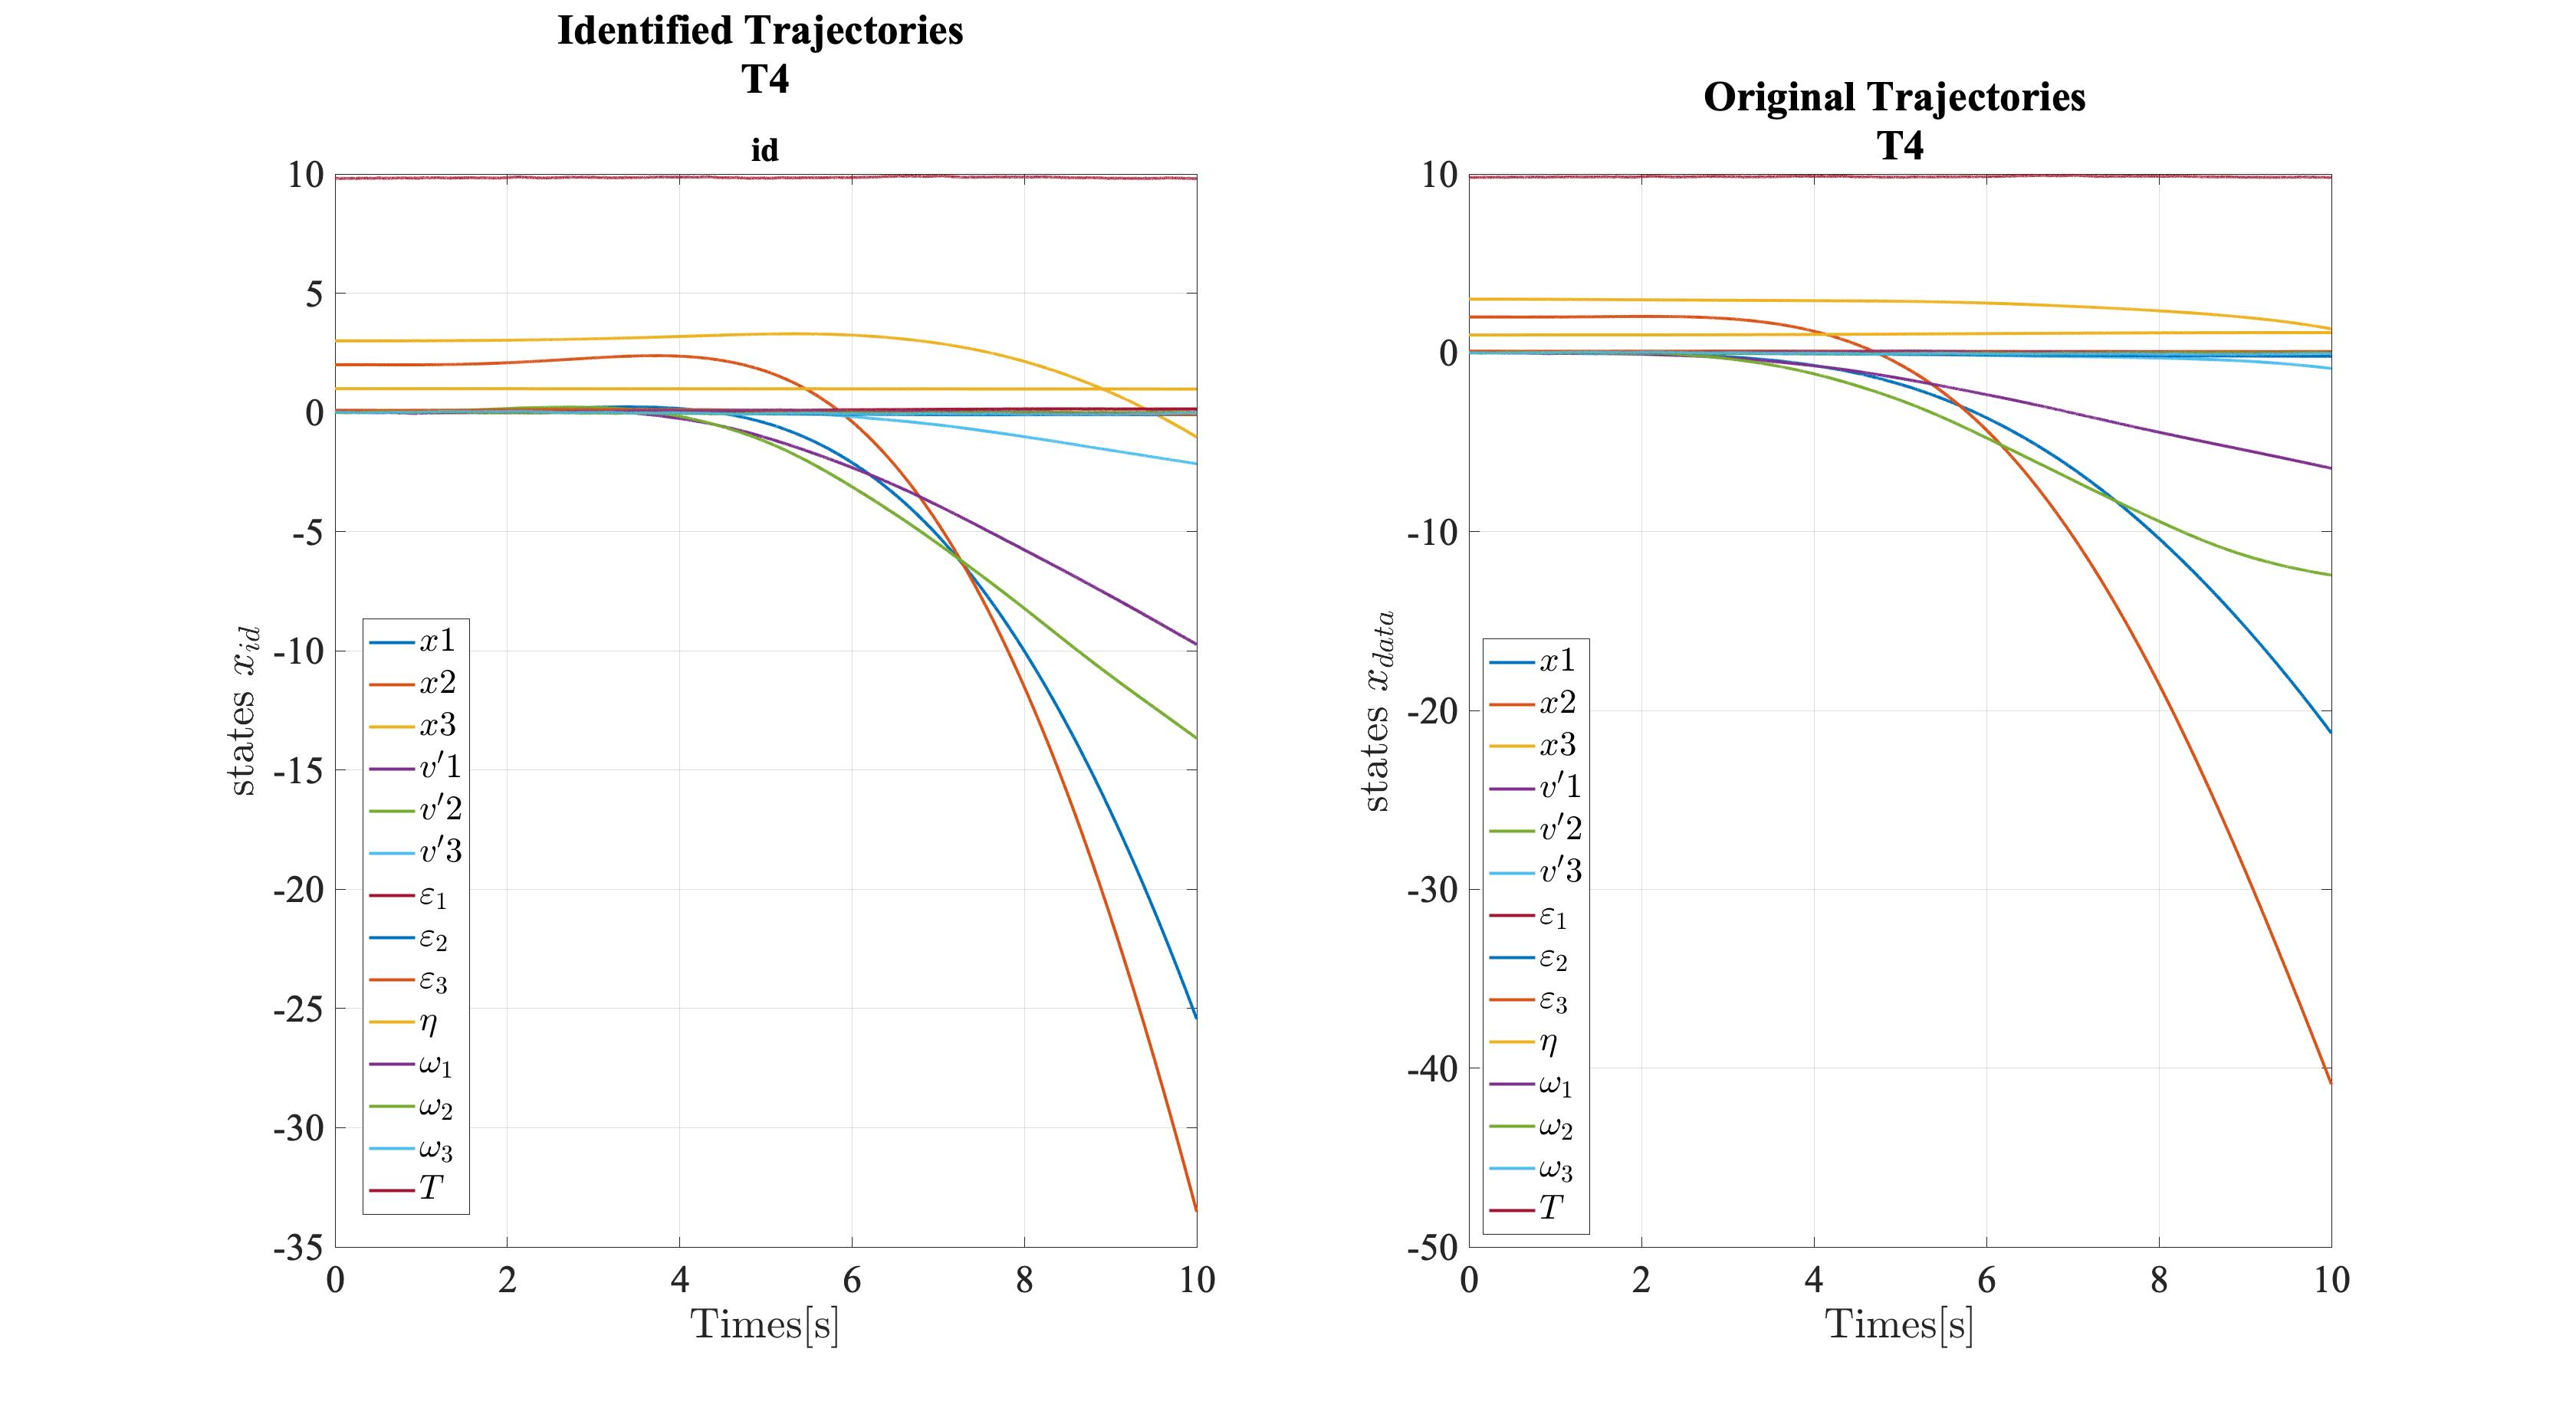
\includegraphics[height=0.30\textwidth]{T4}
        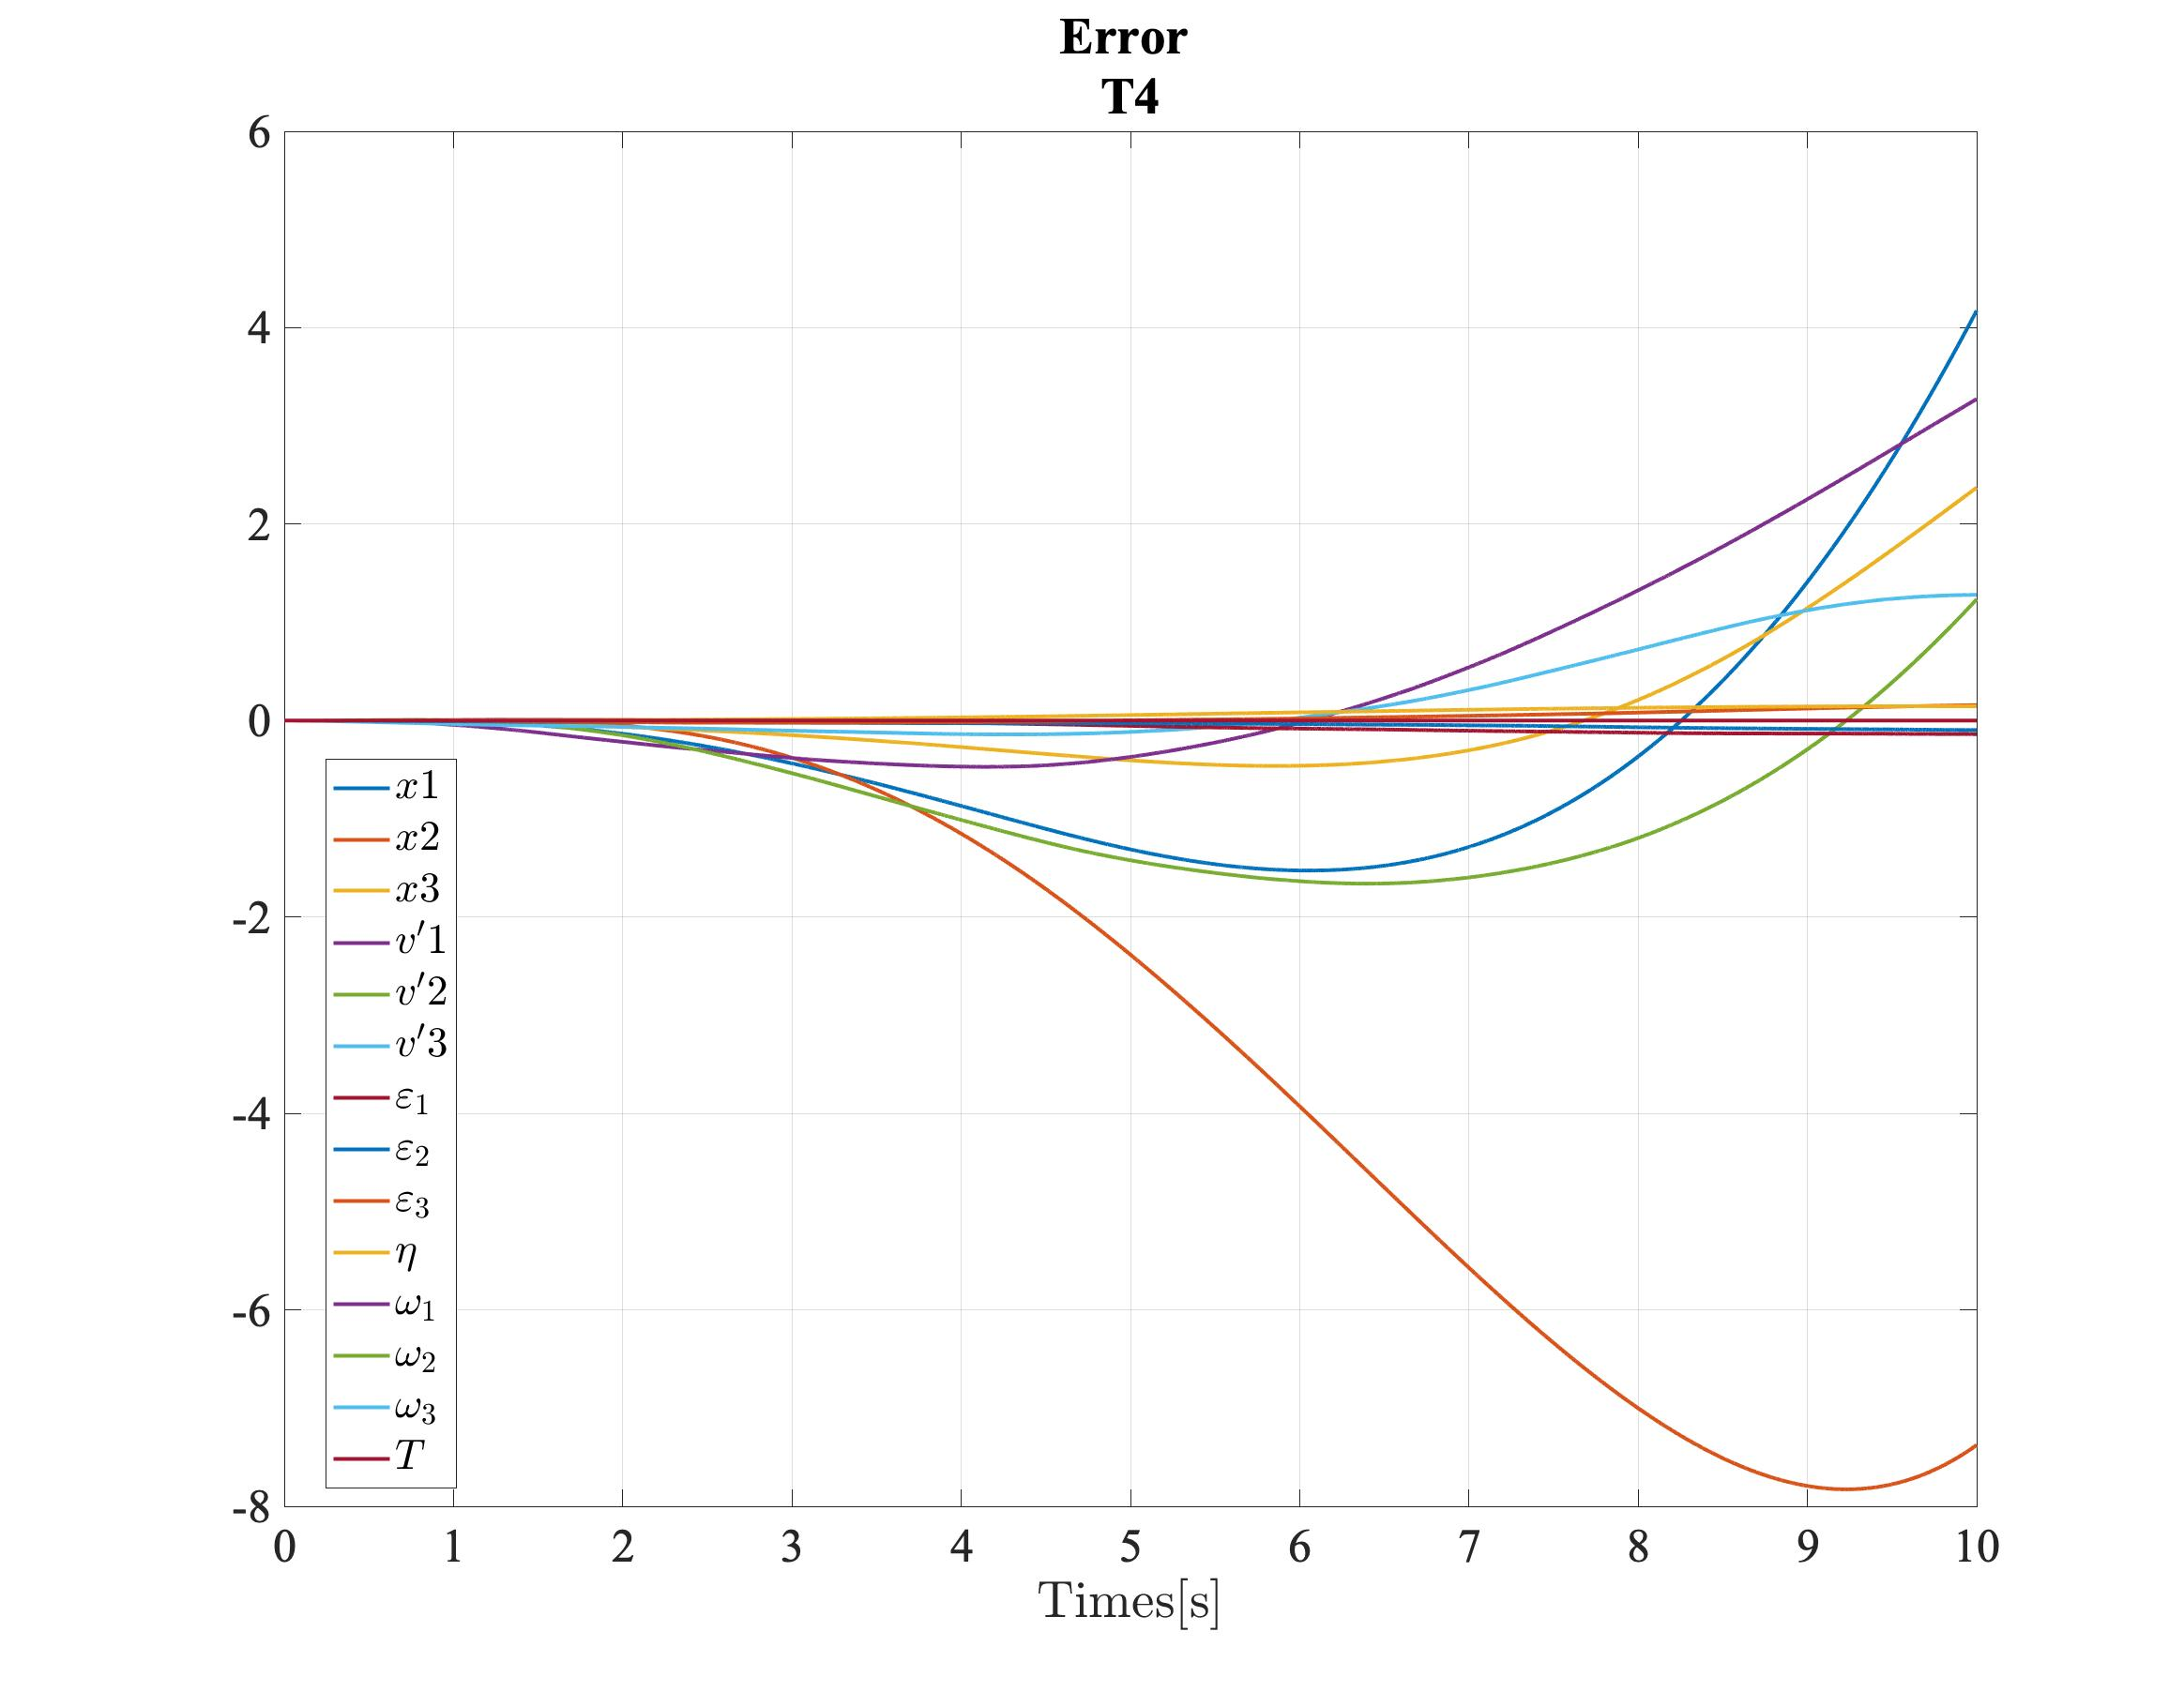
\includegraphics[height=0.30\textwidth]{T4_error}
        \caption{Linearized vs Real System}
        \label{fig:t4}
    \end{figure}
\end{frame}
\begin{frame}
    \frametitle{T5}
    \begin{equation*}
        \begin{array}{c}
            \epsilon = [0, 0, \sin(10)] \\
            \eta = \cos(10)
        \end{array}
    \end{equation*}
    \begin{figure}[htp]
        \centering
        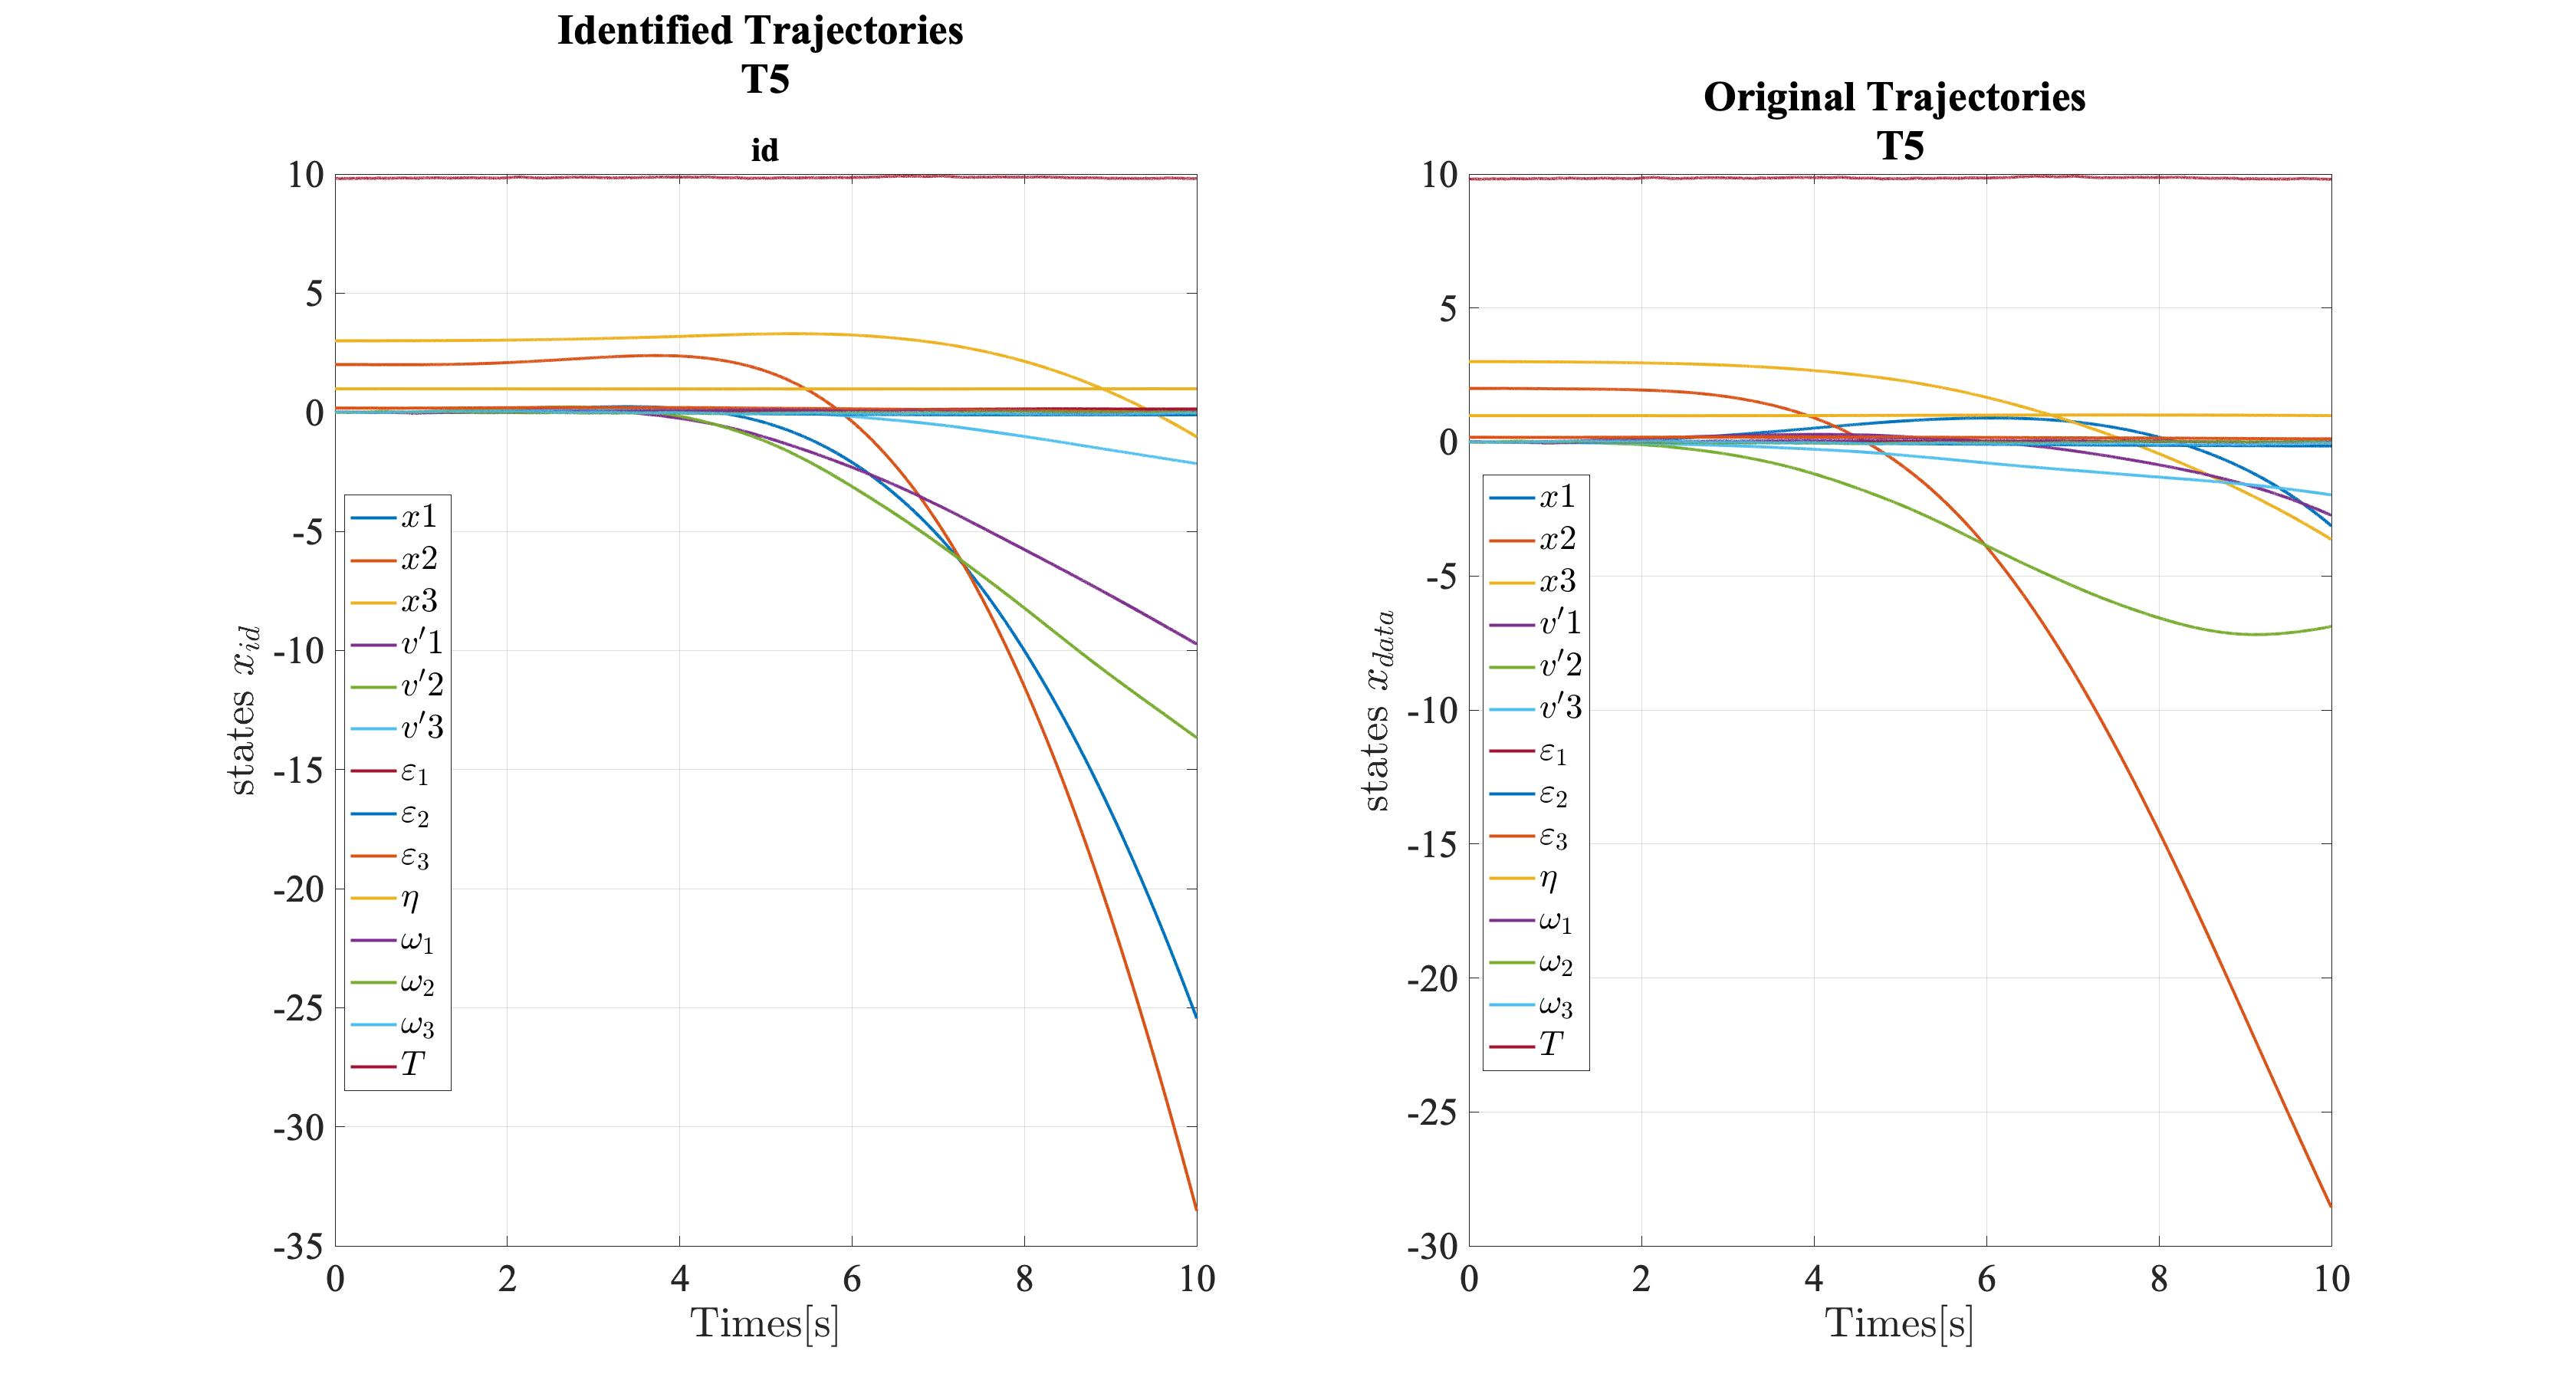
\includegraphics[height=0.30\textwidth]{T5}
        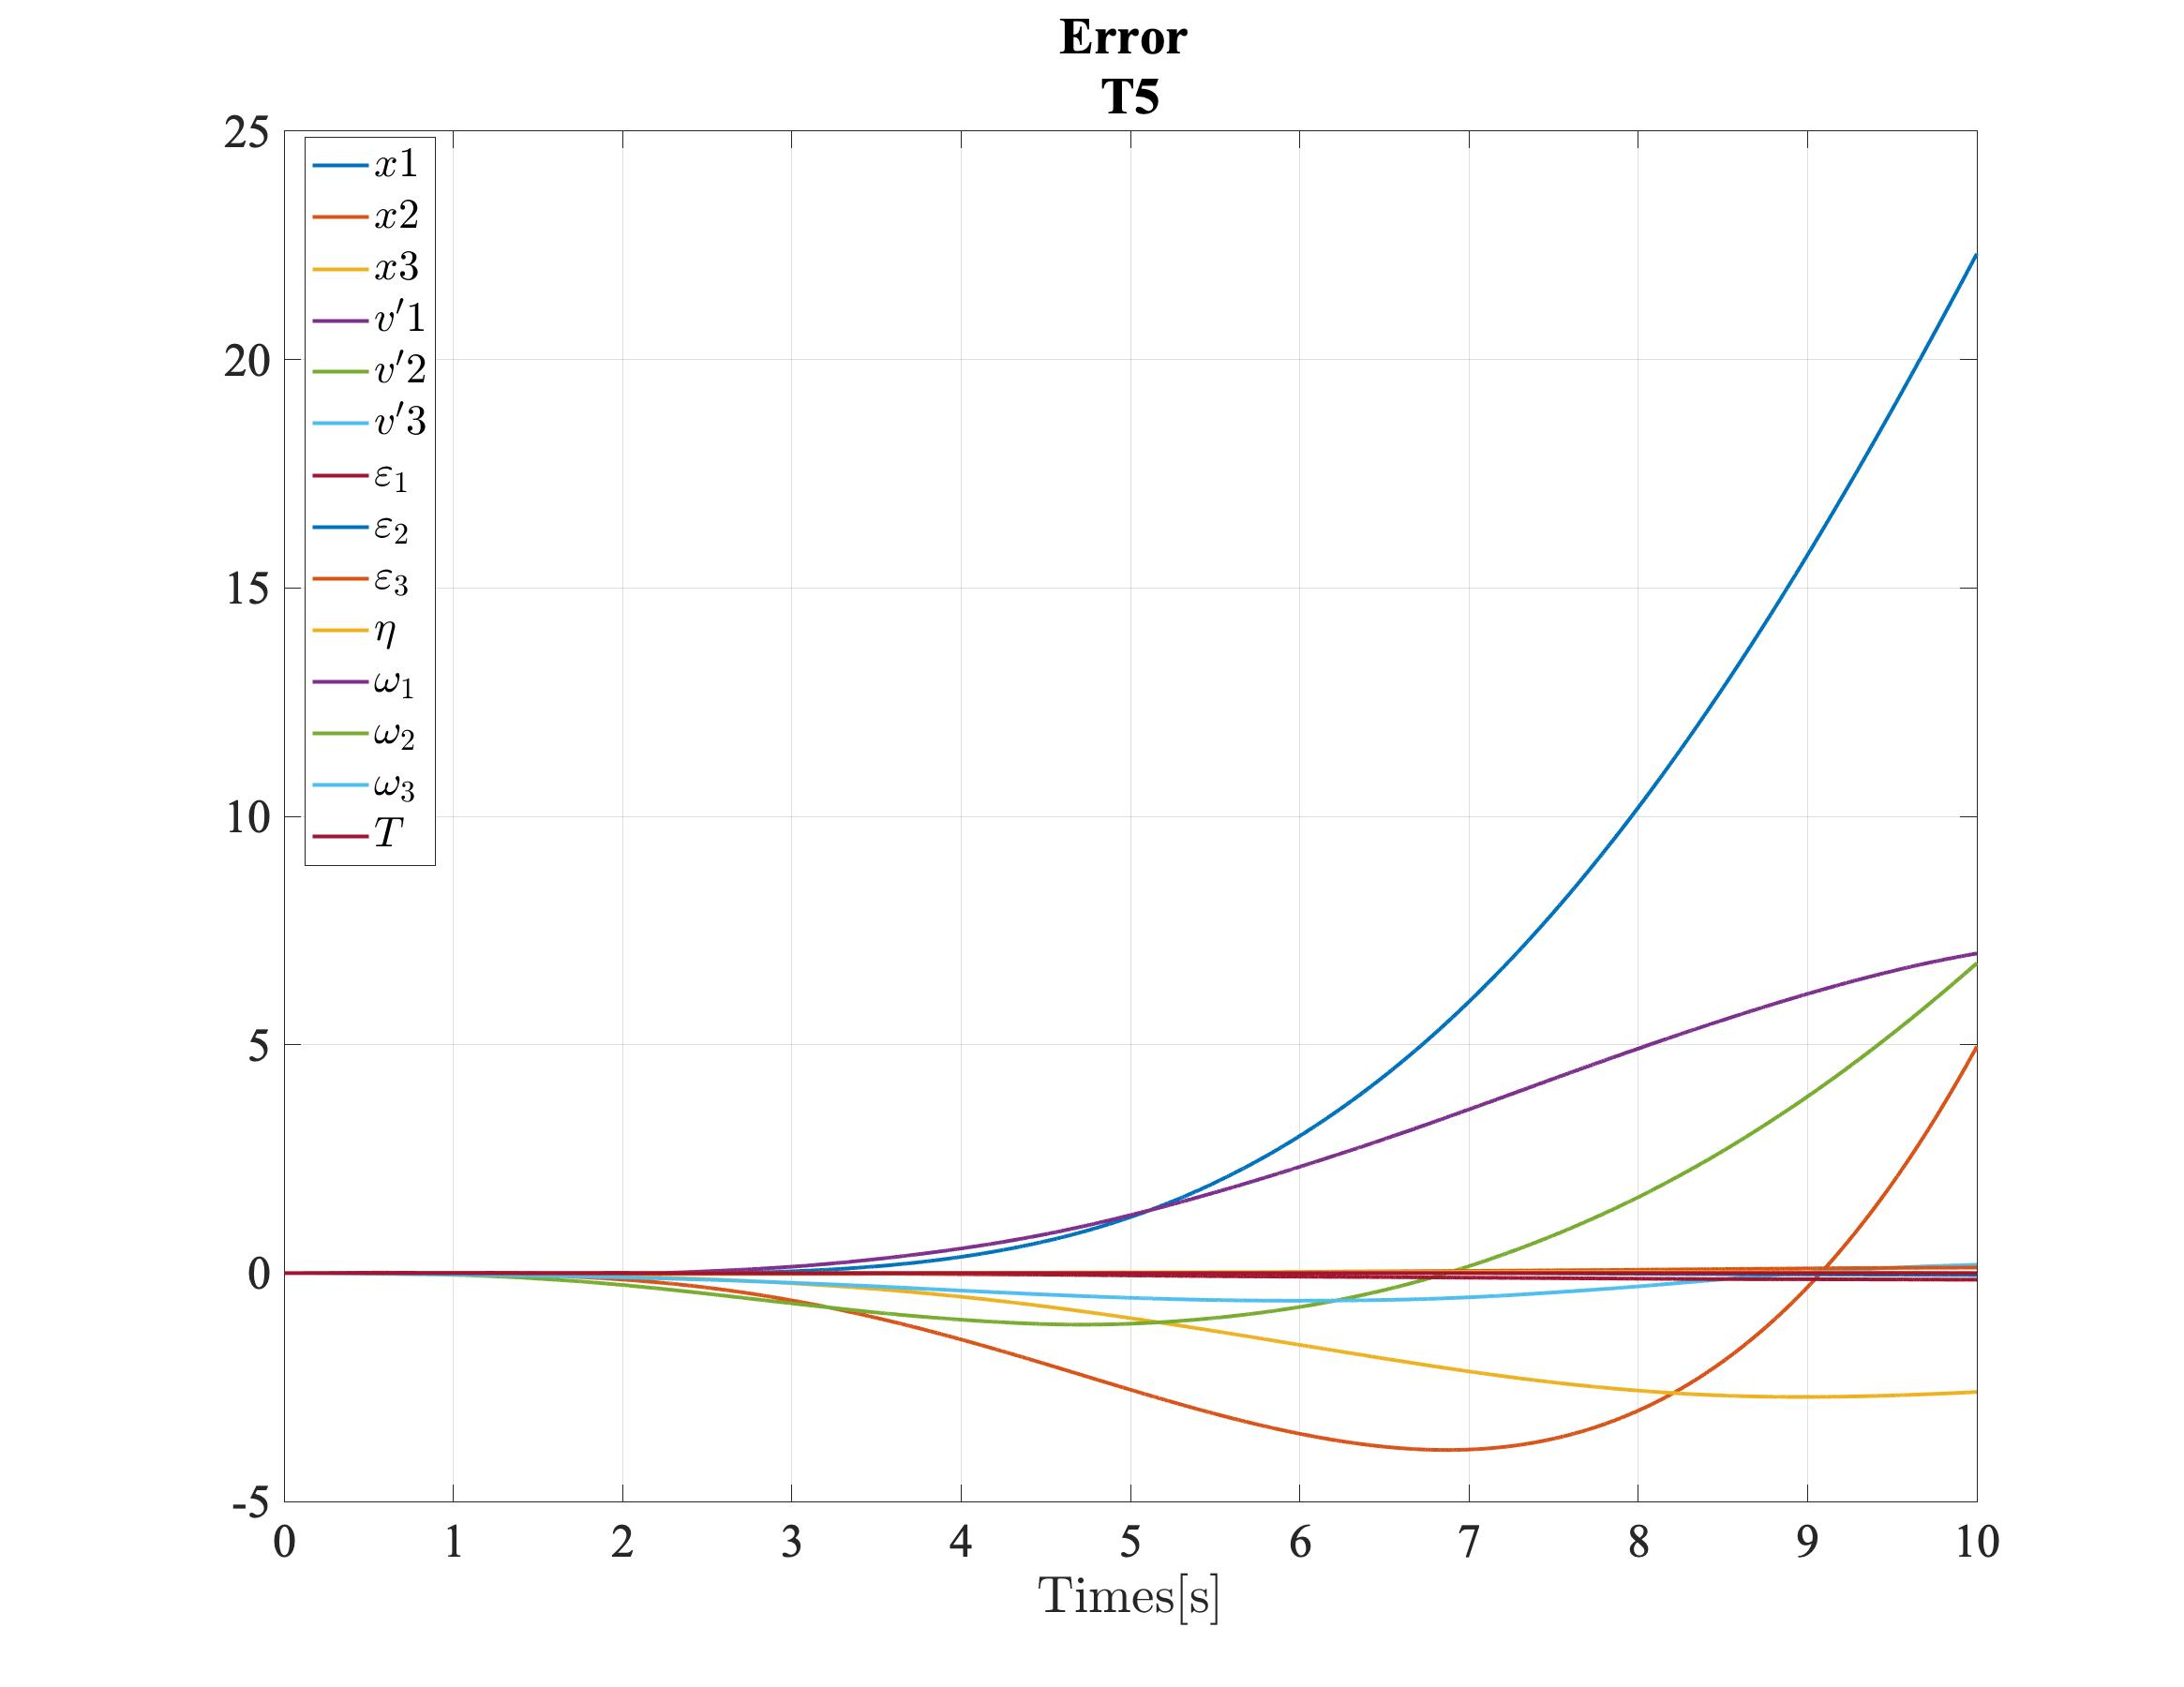
\includegraphics[height=0.30\textwidth]{T5_error}
        \caption{Linearized vs Real System}
        \label{fig:t5}
    \end{figure}
\end{frame}
%---------------------------------------------------------

\section{LQR Controller Design}

%---------------------------------------------------------
%Highlighting text

\begin{frame}[fragile]{}
    \frametitle{LQR in Matlab}

    \begin{center}
        \begin{minipage}{1\textwidth}
            \begin{minted}[mathescape,
          gobble=2,
        %   linenos,
          fontsize=\large,
          framesep=2mm]{matlab}
          %% Controller Settings 
          Q_x = 2.3e3*[1;1;1];
          Q_v = 1e3*[5;5;5];
          Q_e = .5e3*[1;1;1;2];
          Q_omega =200 * [10;10;10];
          Q_dfl = diag([Q_x;Q_v;Q_e;Q_omega]);
          
          R = 1000 * diag([1;1;1;1]);
          C_z = [eye(13,13),zeros(13,25)];
          K = lqr(A,B,C_z'*Q_dfl*C_z,R);
        \end{minted}
        \end{minipage}
    \end{center}

\end{frame}

%---------------------------------------------------------

\begin{frame}
    \frametitle{LQR Parameters}

    \begin{columns}
        \column{0.5\textwidth}
        \begin{center}
            \uline{\bfseries {Initial State}}
        \end{center}
        \begin{itemize}
            \item Position: $p_{0}=\left[\begin{array}{lll}0 & 2 & 3\end{array}\right]^{T}$
            \item Velocity: $v_{0}=\left[\begin{array}{lll}0 & 0 & 0\end{array}\right]^{T}$
            \item Orientation: $\epsilon_{0}=\left[\begin{array}{lll}0 & 0 & \sin 10\end{array}\right]^{T}, \eta_{0}=\cos 10$
            \item Angular Velocity: $\omega_{0}=\left[\begin{array}{lll}0 & 0 & 0\end{array}\right]^{T}$
            \item Thrust: $T_{0}=9.81$
        \end{itemize}
        \column{0.5\textwidth}
        \begin{center}
            \uline{\bfseries {Desired State}}
        \end{center}
        \begin{itemize}
            \item Position: $p=\left[\begin{array}{lll}0 & 0 & 0\end{array}\right]^{T}$
            \item Velocity: $v=\left[\begin{array}{lll}0 & 0 & 0\end{array}\right]^{T}$
            \item Orientation: $\epsilon=\left[\begin{array}{lll}0 & 0 & 0\end{array}\right]^{T}, \eta=1 $
            \item Angular Velocity: $\omega=\left[\begin{array}{lll}0 & 0 & 0\end{array}\right]^{T}$
            \item Thrust: $T=9.81$
        \end{itemize}
    \end{columns}
\end{frame}
%---------------------------------------------------------
%Two columns
\subsection{Results}

\begin{frame}
    \frametitle{Postion and Velocity}

    \begin{columns}

        \column{0.5\textwidth}
        \begin{figure}[h]
            \centering
            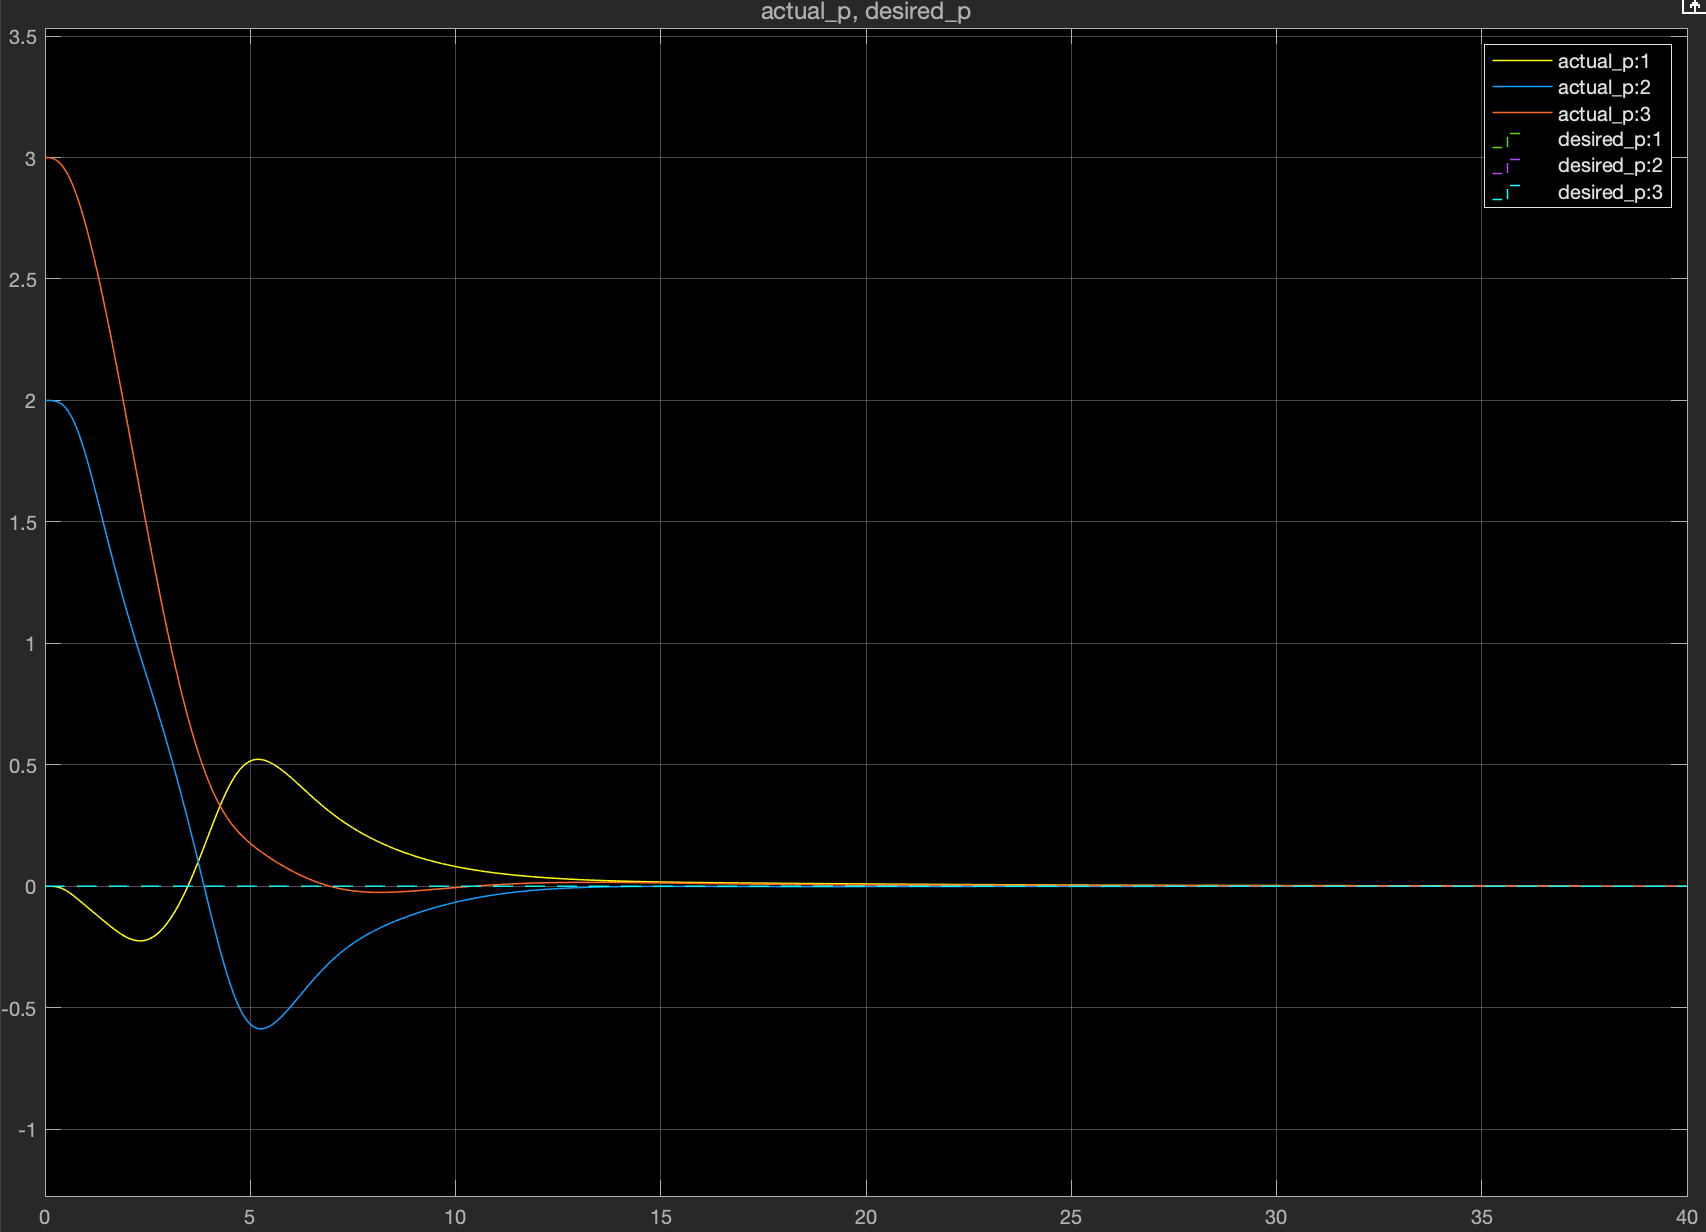
\includegraphics[width=1\textwidth]{position.png}
            \caption{Position plot}
            \label{fig:postion}
        \end{figure}

        \column{0.5\textwidth}
        \begin{figure}[h]
            \centering
            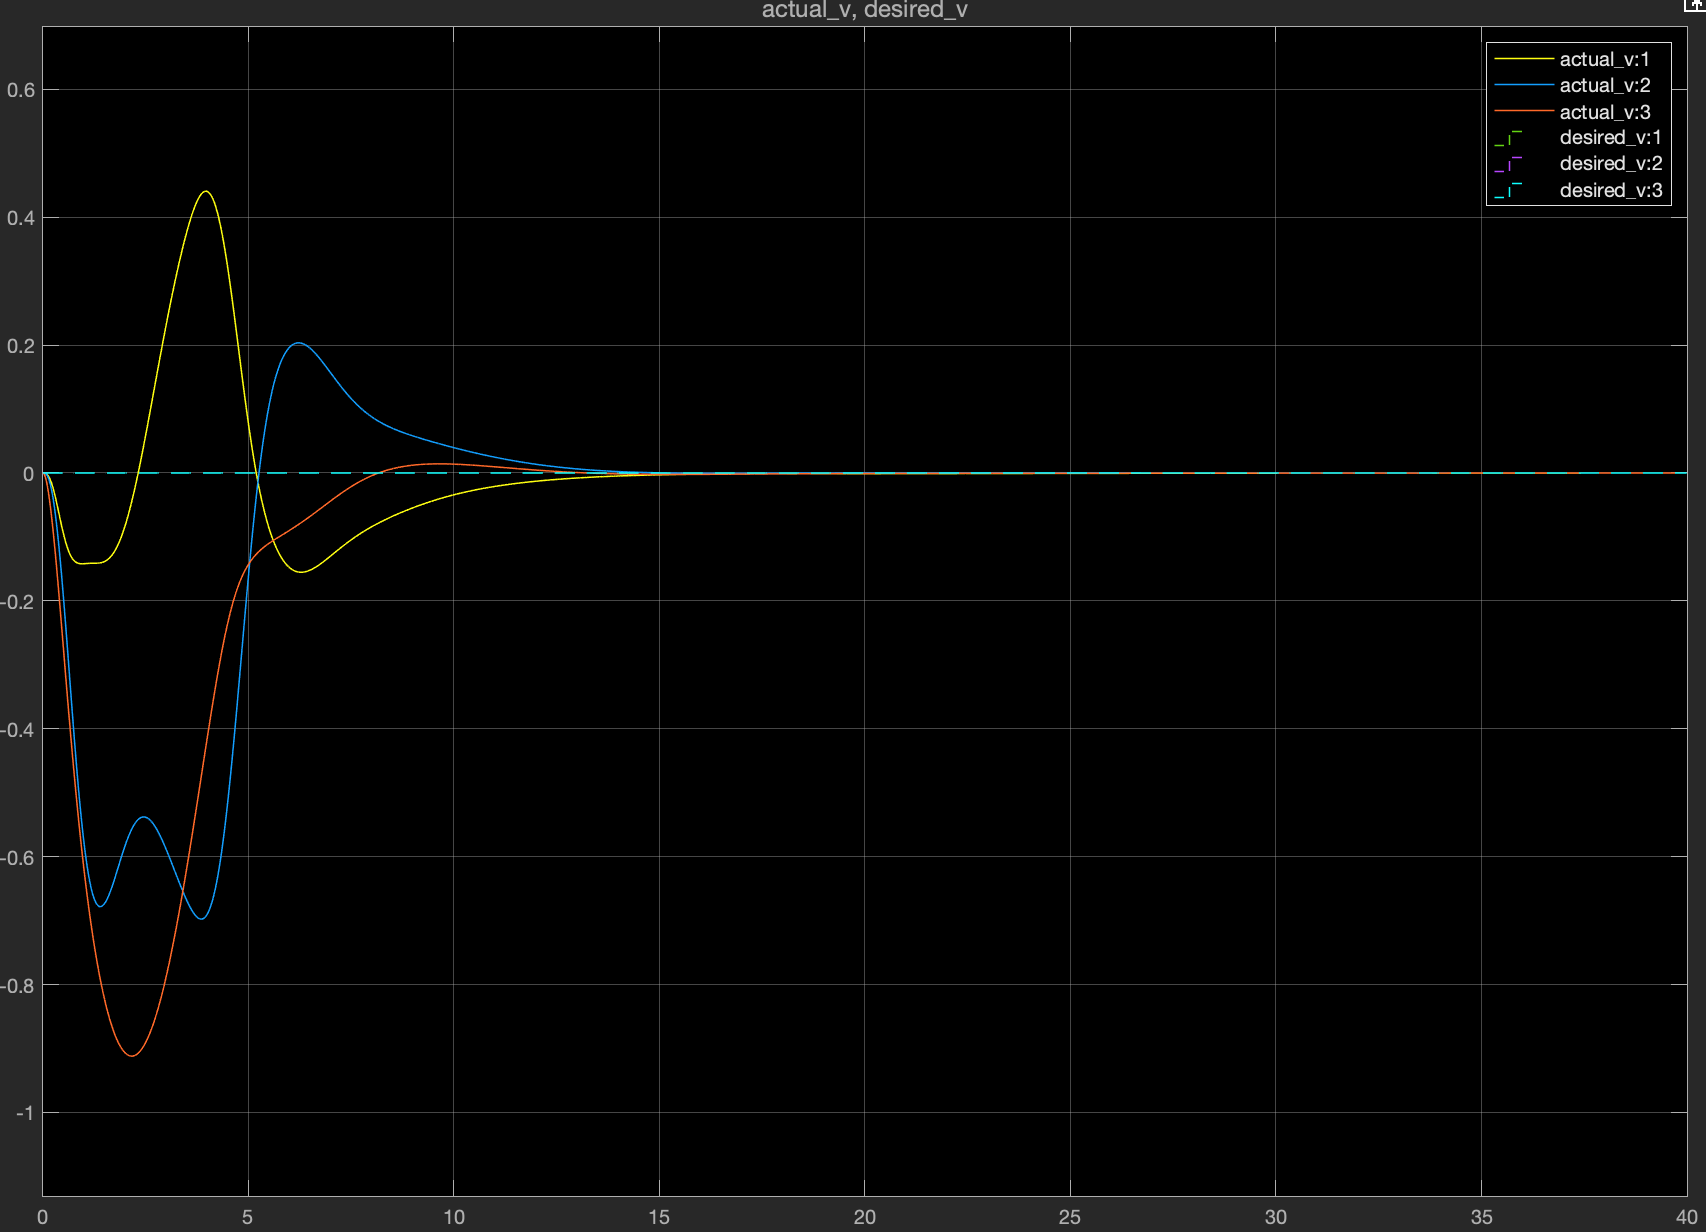
\includegraphics[width=1\textwidth]{velocity.png}
            \caption{Velocity plot}
            \label{fig:velocity}
        \end{figure}
    \end{columns}
\end{frame}

\begin{frame}
    \frametitle{Euler Parameters}

    \begin{columns}

        \column{0.5\textwidth}
        \begin{figure}[h]
            \centering
            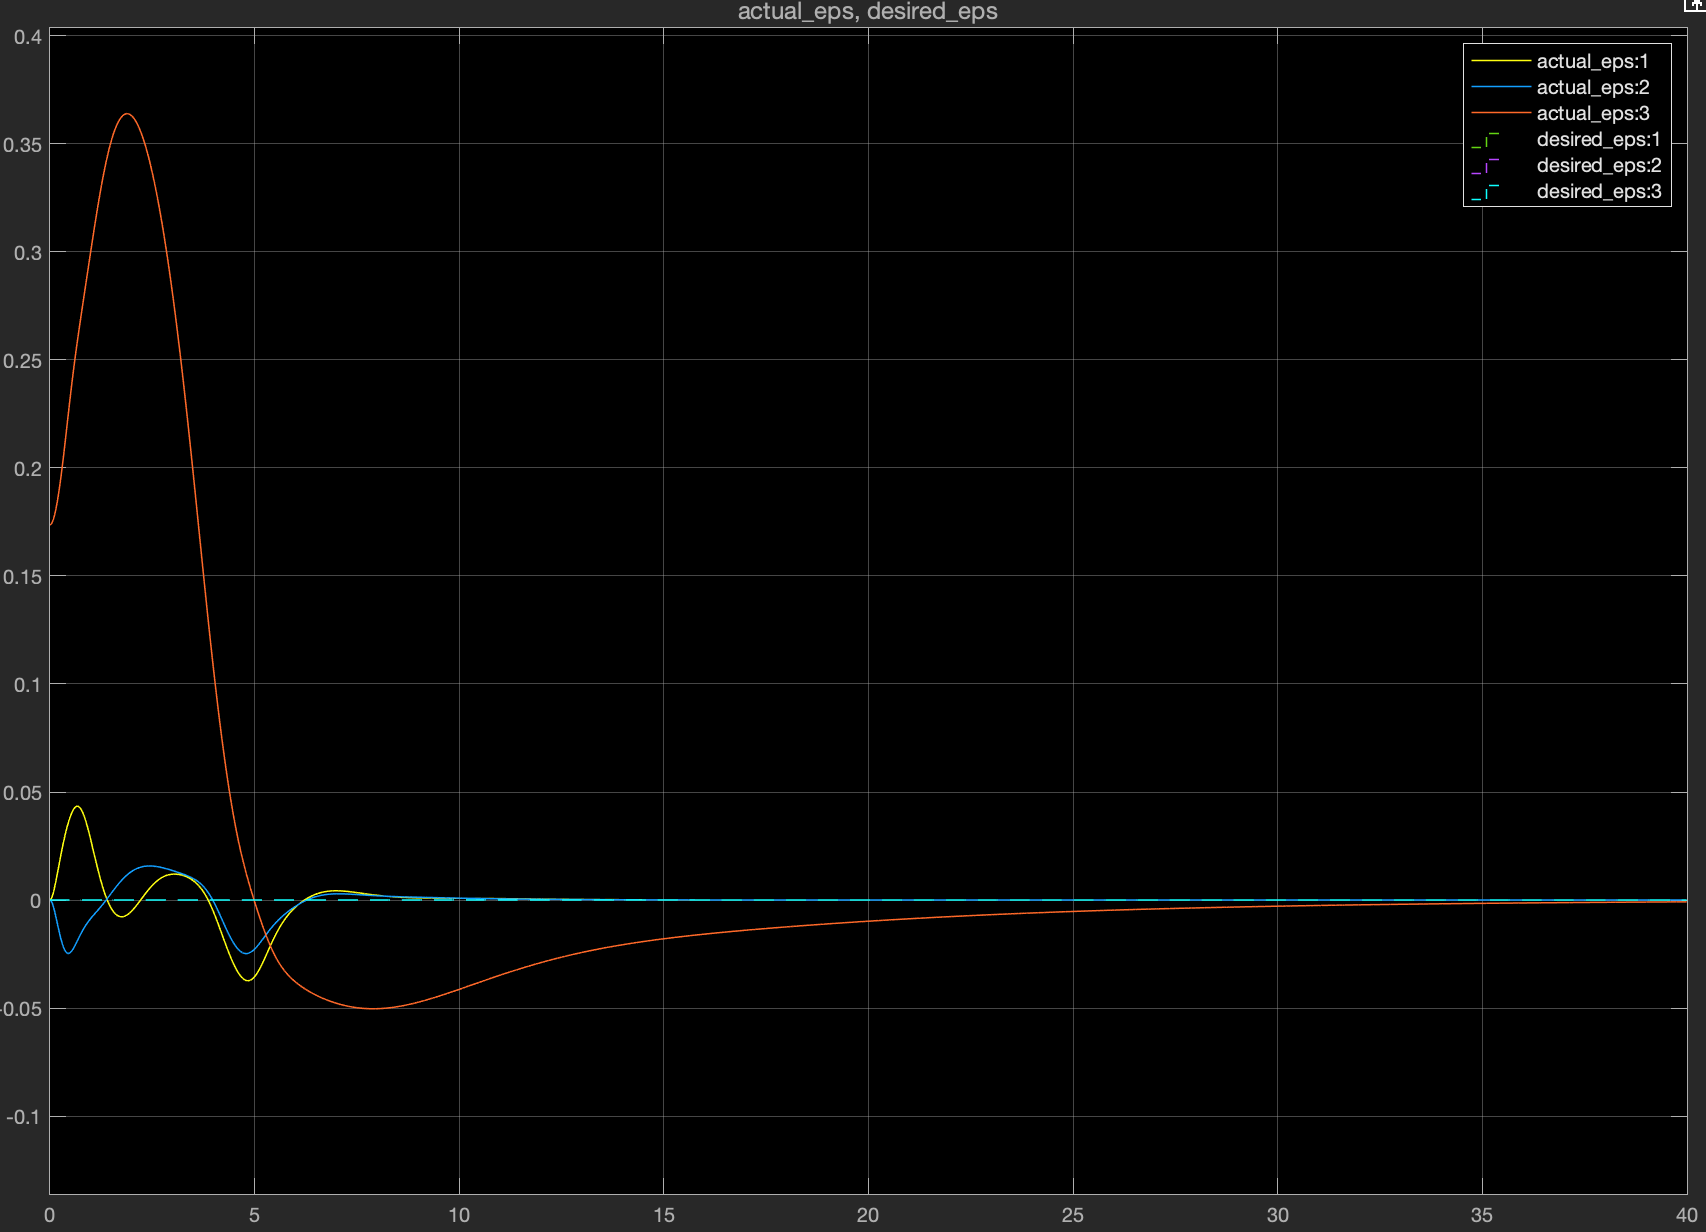
\includegraphics[width=1\textwidth]{epsilon.png}
            \caption{Epsilon plot}
            \label{fig:epsilon}
        \end{figure}

        \column{0.5\textwidth}
        \begin{figure}[h]
            \centering
            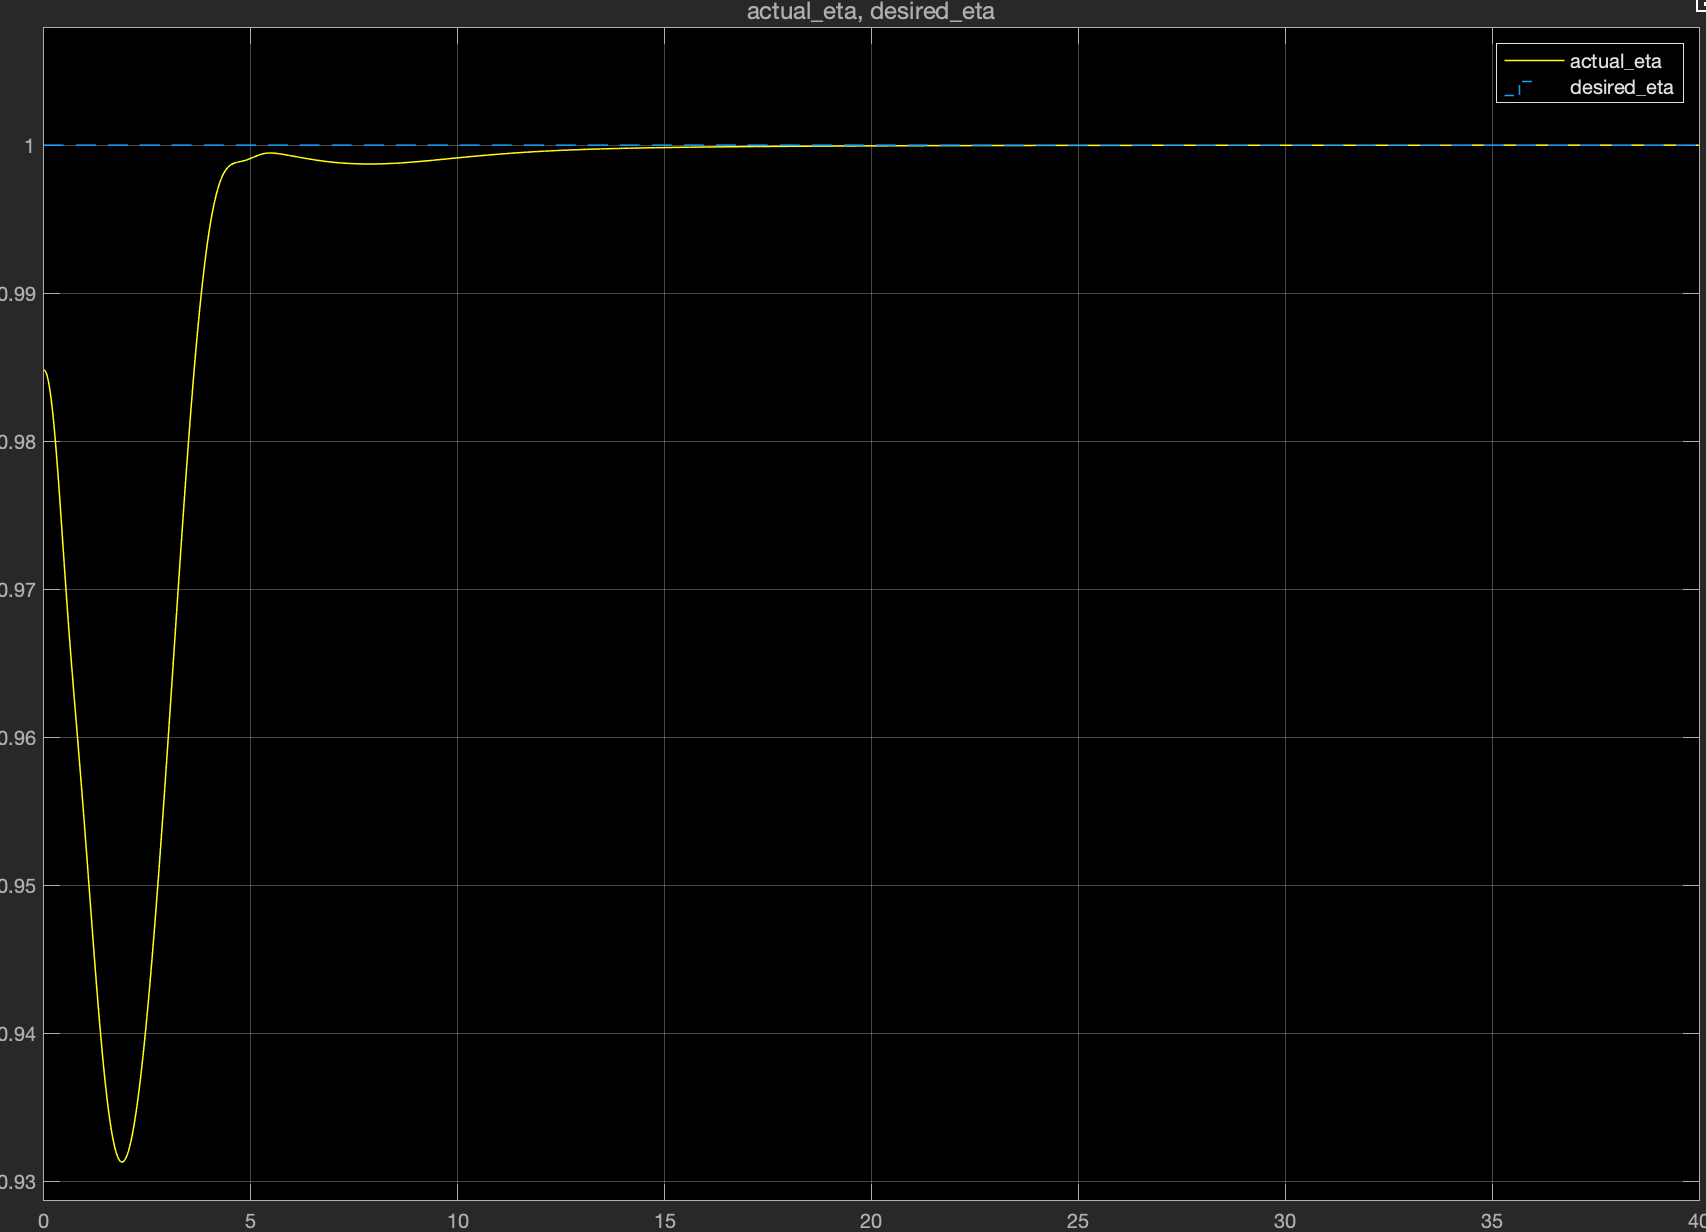
\includegraphics[width=1\textwidth]{eta.png}
            \caption{eta plot}
            \label{fig:eta}
        \end{figure}
    \end{columns}
\end{frame}

\begin{frame}
    \frametitle{Angular Velocity and Inputs}

    \begin{columns}

        \column{0.5\textwidth}
        \begin{figure}[h]
            \centering
            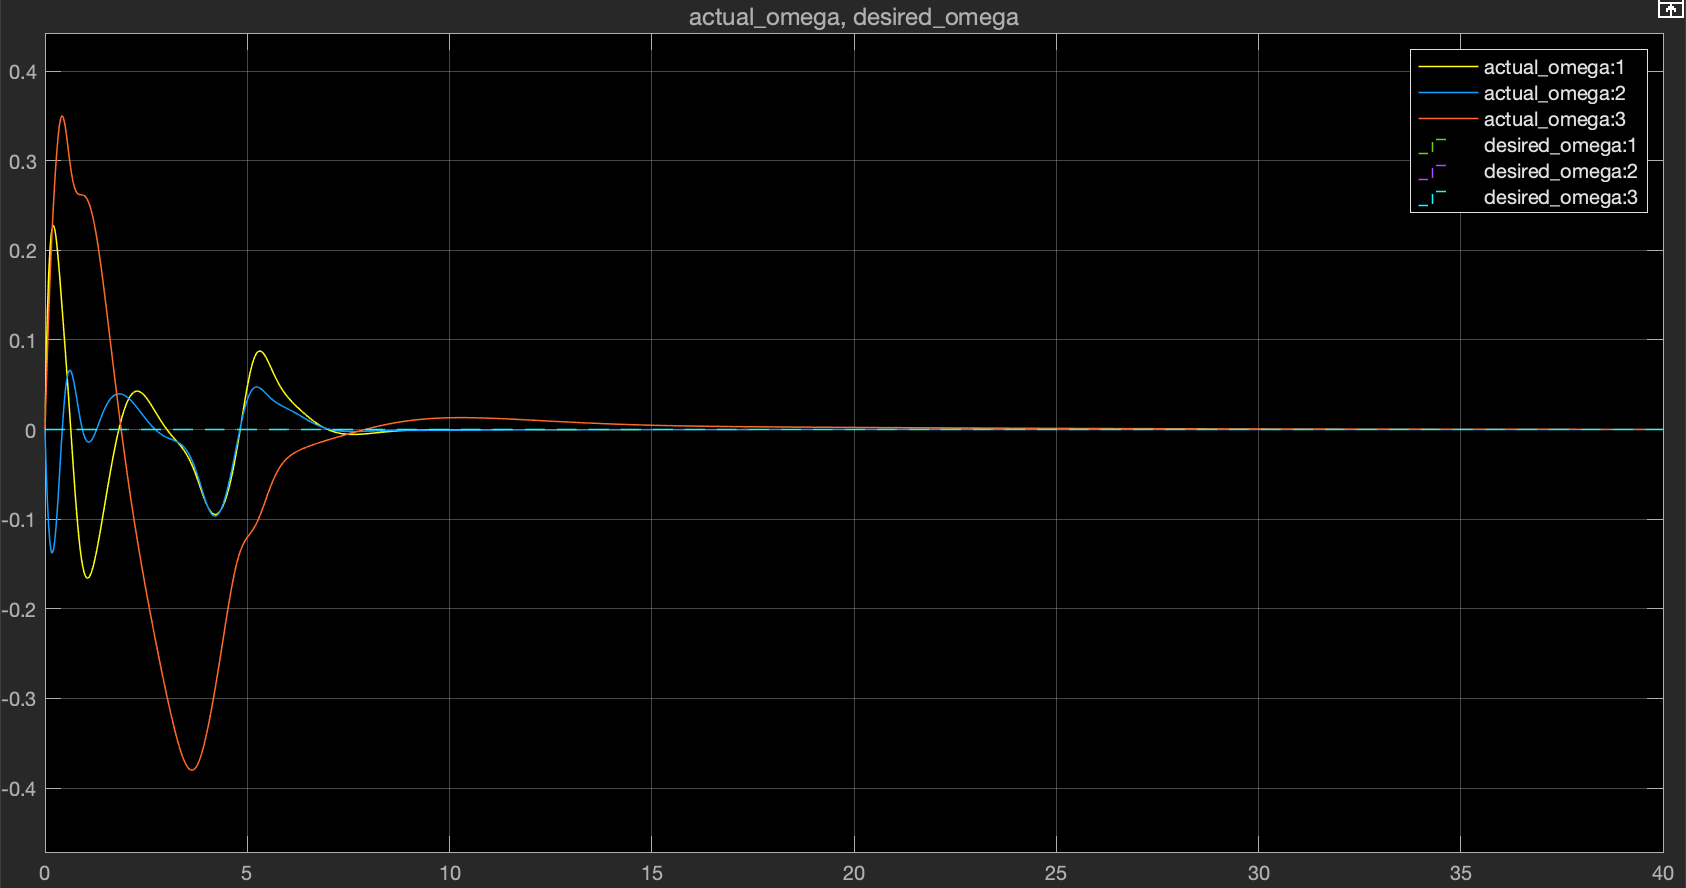
\includegraphics[width=1\textwidth]{omega.png}
            \caption{Angular Velocity plot}
            \label{fig:omega}
        \end{figure}

        \column{0.5\textwidth}
        \begin{figure}[h]
            \centering
            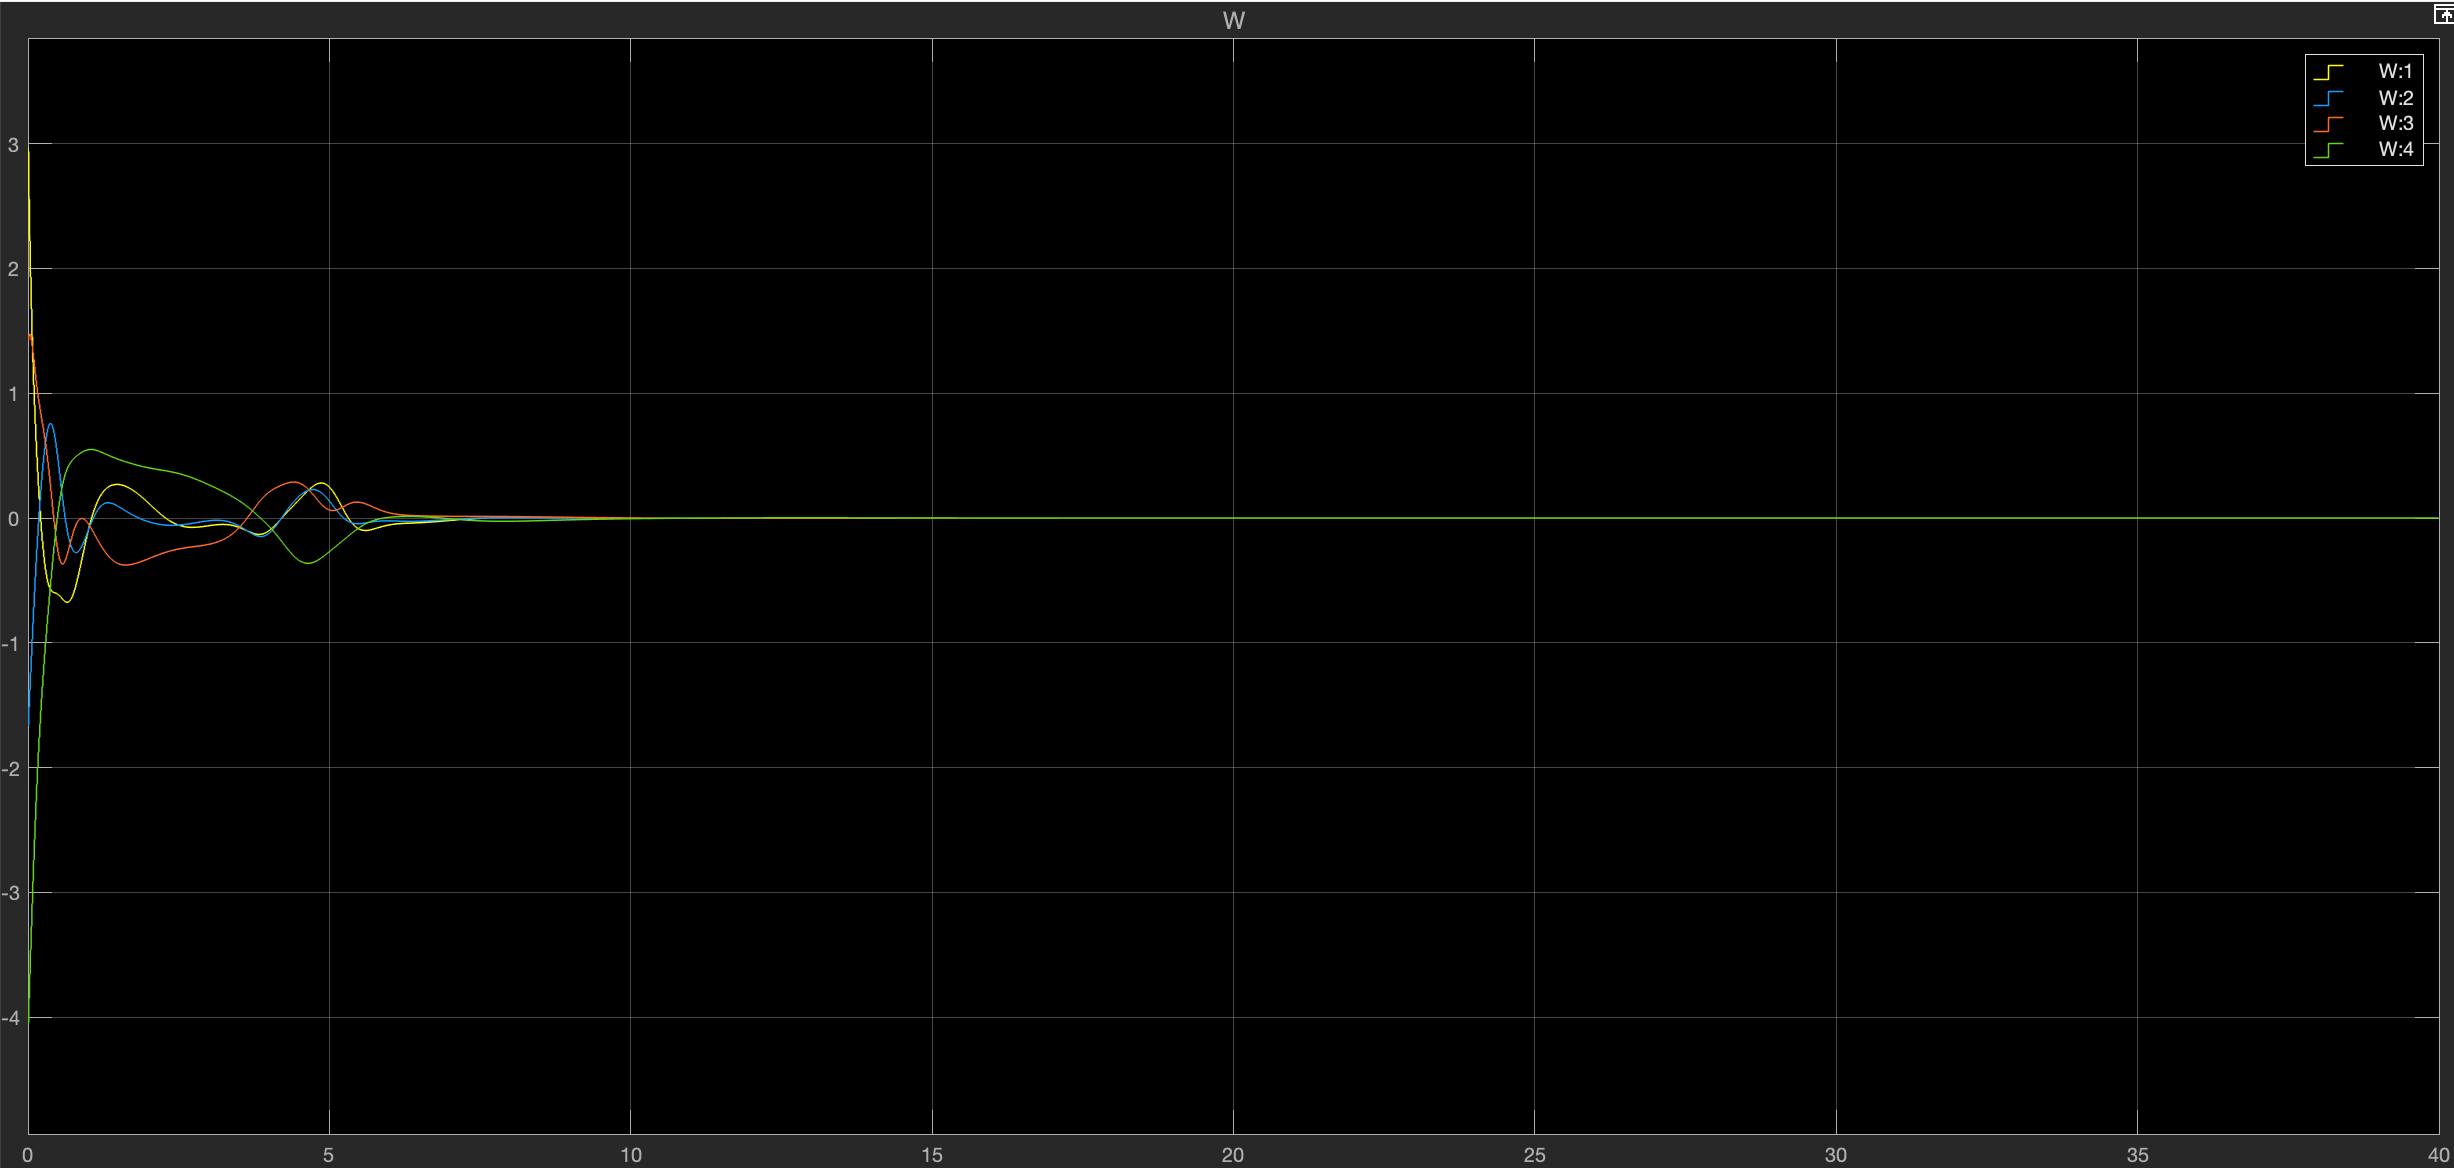
\includegraphics[width=1\textwidth]{Inputs.png}
            \caption{Inputs plot}
            \label{fig:inputs}
        \end{figure}
    \end{columns}
\end{frame}

\begin{frame}
    \frametitle{Auxiliary Parameters}

    \begin{columns}

        \column{0.5\textwidth}
        \begin{figure}[h]
            \centering
            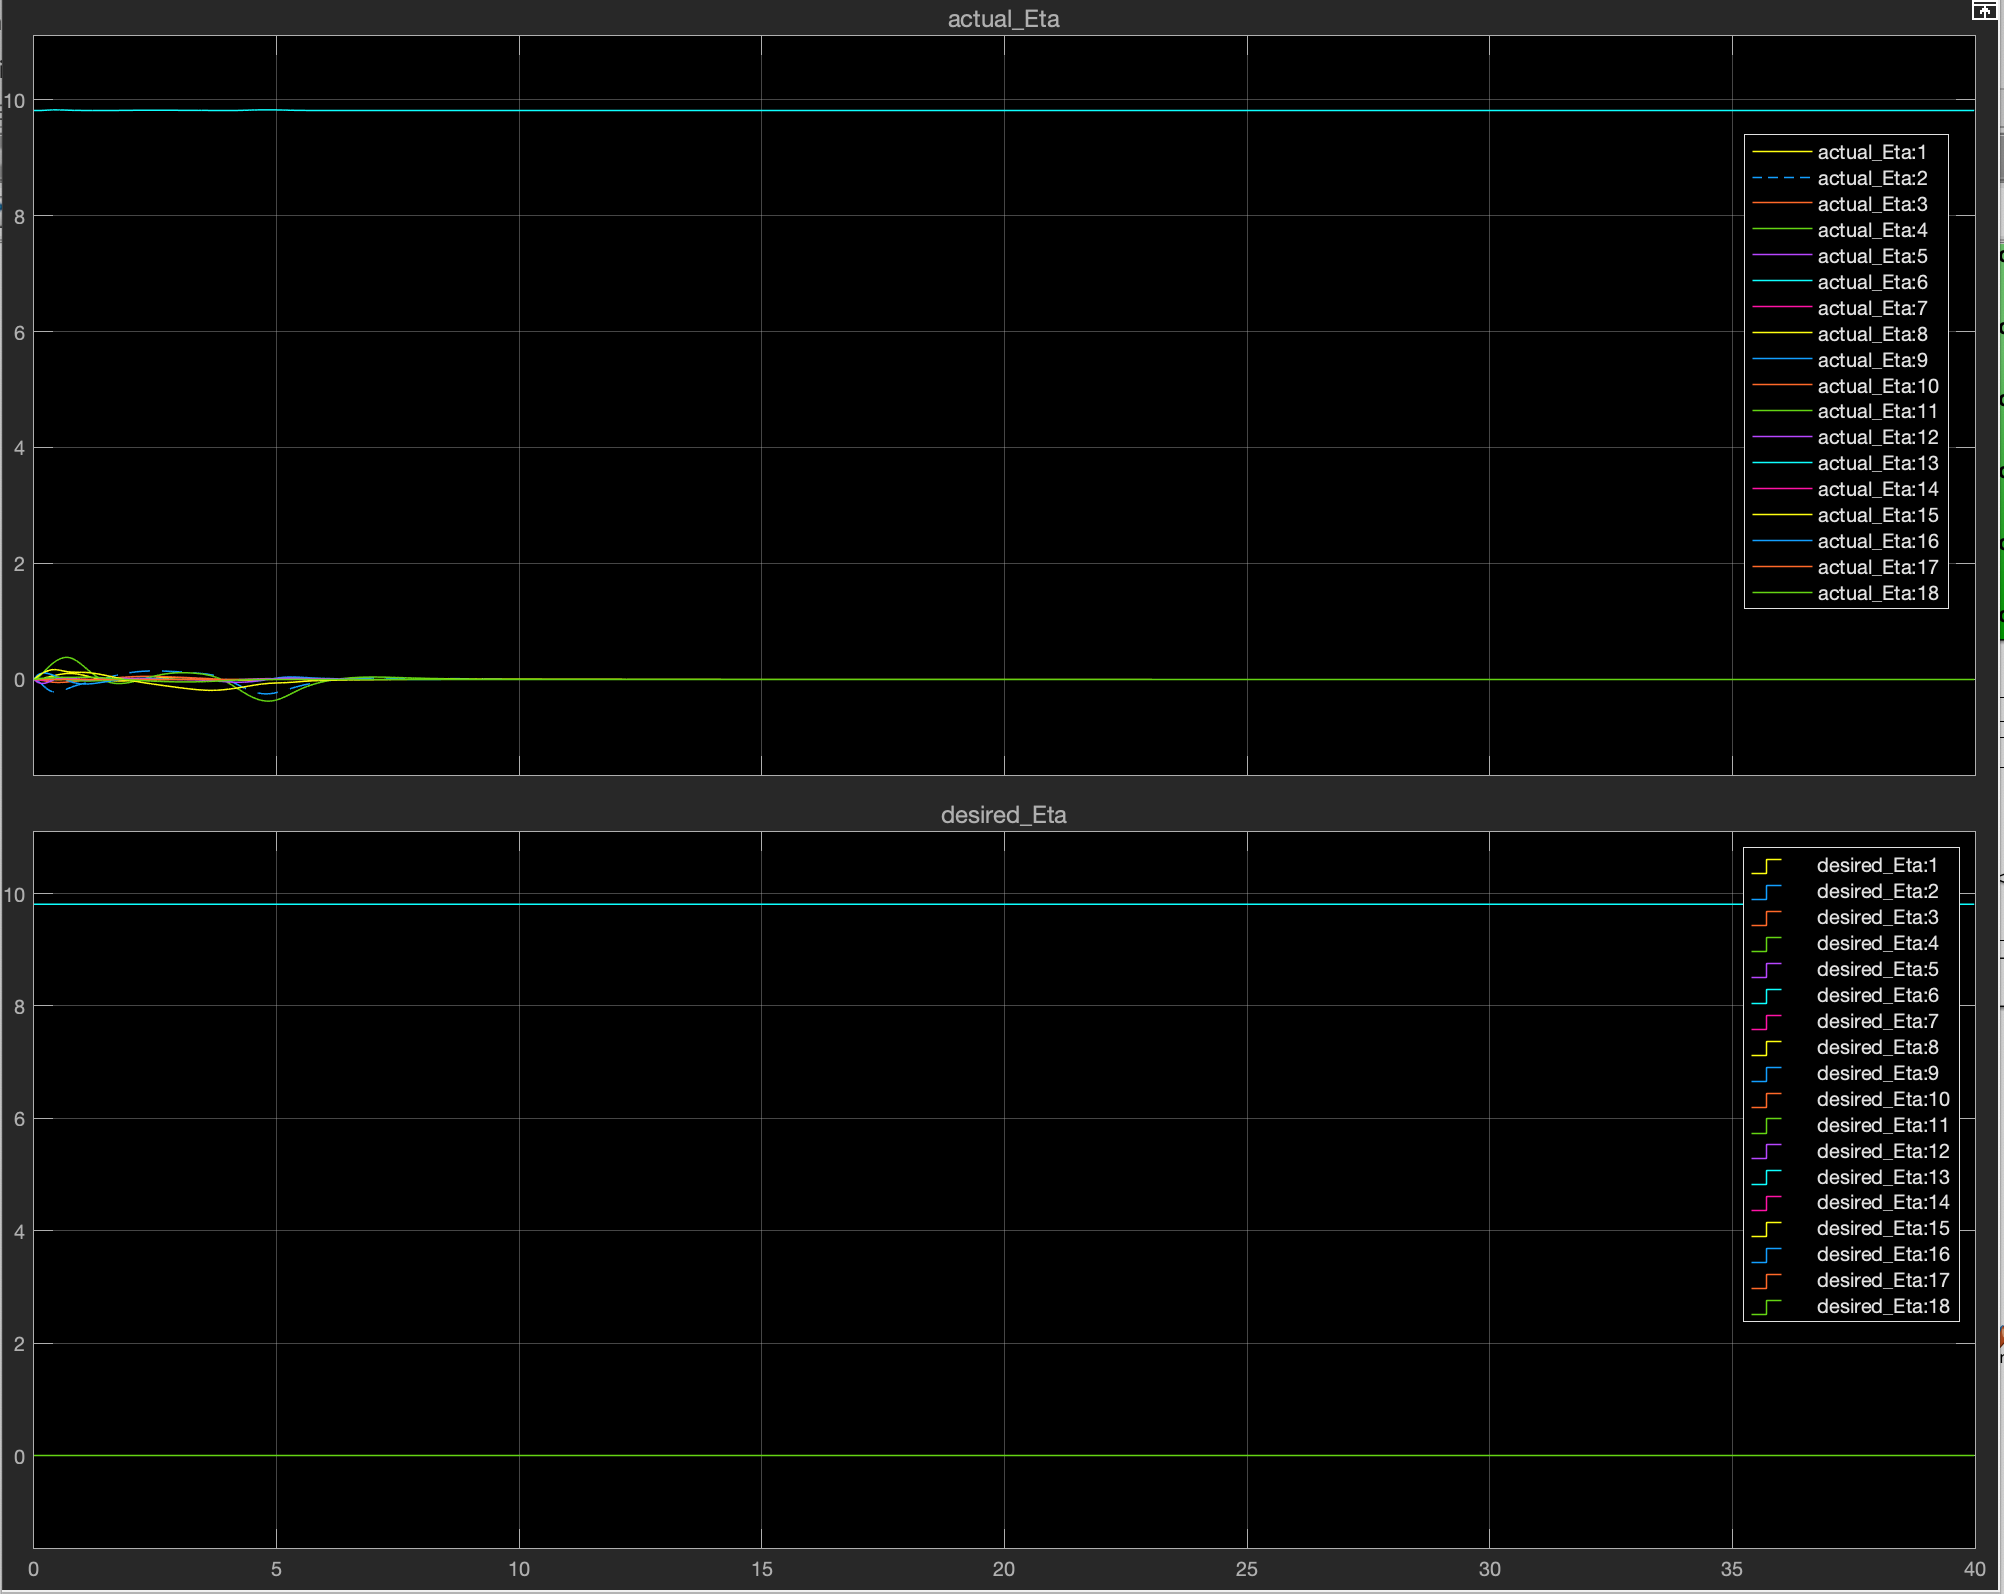
\includegraphics[width=1\textwidth]{Etas.png}
            \caption{Etas plot}
            \label{fig:etas}
        \end{figure}

        \column{0.5\textwidth}
        \begin{figure}[h]
            \centering
            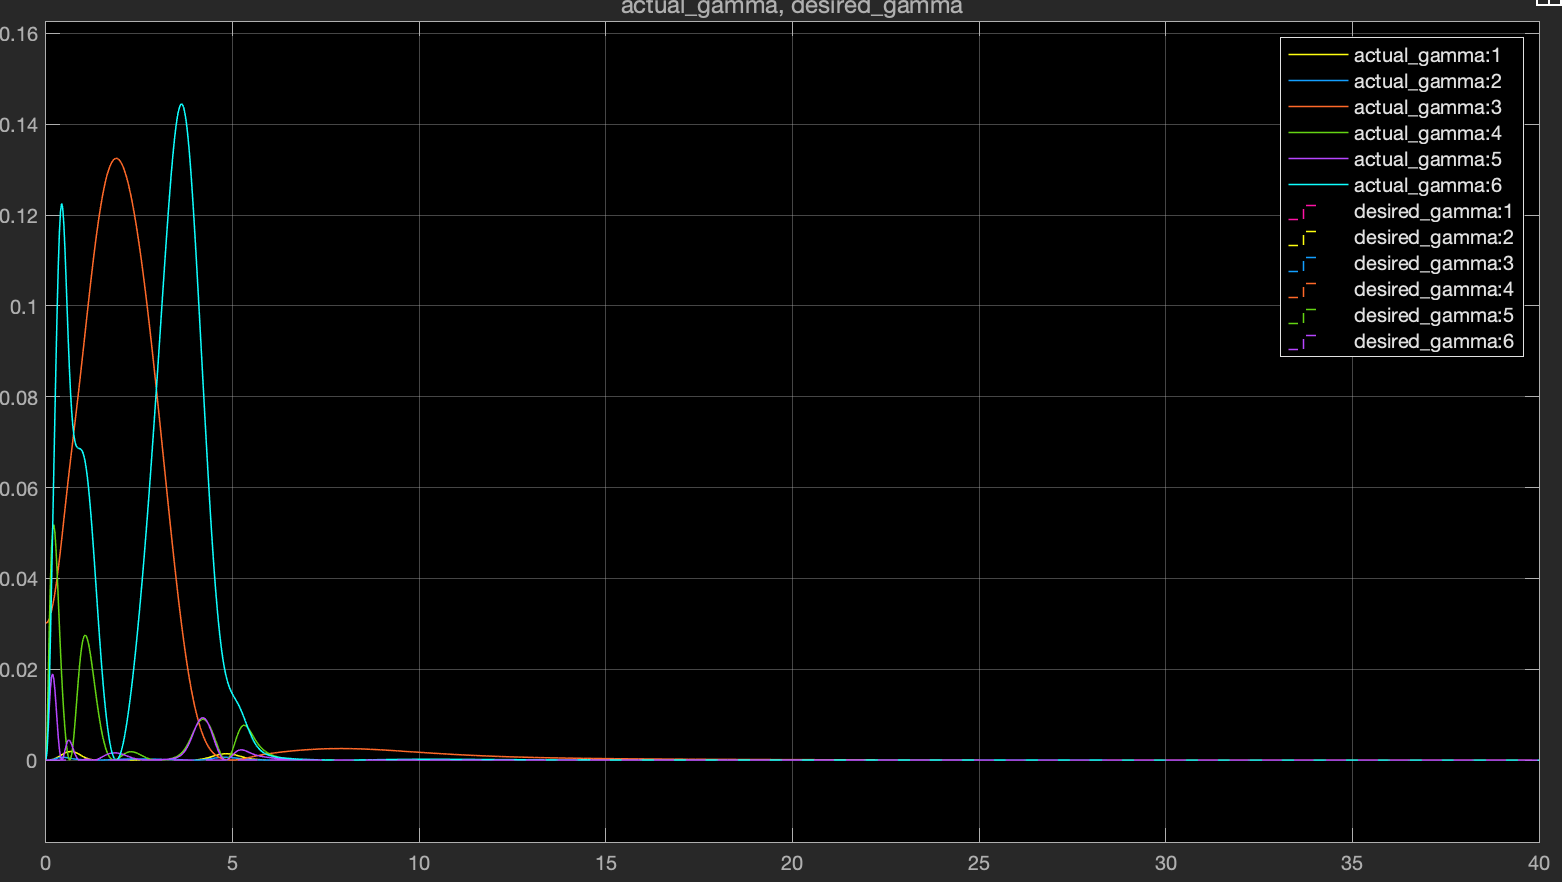
\includegraphics[width=1\textwidth]{Gamma.png}
            \caption{Gamma plot}
            \label{fig:gamma}
        \end{figure}
    \end{columns}
\end{frame}


%---------------------------------------------------------


\section{Taylor Linearization}
\begin{frame}
    \begin{equation*}
        \dot{x}=\left(\begin{array}{c}
                \dot{p_{1}}        \\
                \dot{p_{2}}        \\
                \dot{p_{3}}        \\
                \dot{v_{1}}        \\
                \dot{v_{2}}        \\
                \dot{v_{3}}        \\
                \dot{\epsilon_{1}} \\
                \dot{\epsilon_{2}} \\
                \dot{\epsilon_{3}} \\
                \dot{\eta}         \\
                \dot{\omega_{1}}   \\
                \dot{\omega_{2}}   \\
                \dot{\omega_{3}}   \\
                \dot{T}
            \end{array}\right)=\left(\begin{array}{c}
                v_{1}                                                                                                  \\
                v_{2}                                                                                                  \\
                v_{3}                                                                                                  \\
                T\left(2 \epsilon_{1} \epsilon_{3}+2 \epsilon_{2} \eta\right)                                          \\
                T\left(2 \epsilon_{2} \epsilon_{3}-2 \epsilon_{1} \eta\right)                                          \\
                9.81-T\left(2 \epsilon_{1}^{2}+2 \epsilon_{2}^{2}-1\right)                                             \\
                \frac{\epsilon_{3} \omega_{2}}{2}-\frac{\epsilon_{2} \omega_{3}}{2}+\frac{\eta \omega_{1}}{2}          \\
                \frac{\epsilon_{1} \omega_{3}}{2}-\frac{\epsilon_{3} \omega_{1}}{2}+\frac{\eta \omega_{2}}{2}          \\
                \frac{\epsilon_{2} \omega_{1}}{2}-\frac{\epsilon_{1} \omega_{2}}{2}+\frac{\eta \omega_{3}}{2}          \\
                -\frac{\epsilon_{1} \omega_{1}}{2}-\frac{\epsilon_{2} \omega_{2}}{2}-\frac{\epsilon_{3} \omega_{3}}{2} \\
                w_{1,1}                                                                                                \\
                w_{1,2}                                                                                                \\
                w_{1,3}                                                                                                \\
                w_{2}
            \end{array}\right) = \left(\begin{array}{c}
                0 \\
                0 \\
                0 \\
                0 \\
                0 \\
                0 \\
                0 \\
                0 \\
                0 \\
                0 \\
                0 \\
                0 \\
                0 \\
                0
            \end{array}\right)
    \end{equation*}
    this equilibrium state is reach when
    $\boldsymbol{x}=\left[\begin{array}{llllllllllllll} 0  & 0  & 0  & 0  & 0  & 0  & 0  & 0  & 0  & 1  & 0  & 0  & 0  & 9.81 \end{array}\right]_{14 \times 1}^{T}$
    So this model can be Linearized in the neighborhood

\end{frame}

\begin{frame}
    \frametitle{Linearization}
    Linearization of dynamic equation as $\dot{x}=A x+B u$, where
    \begin{equation}
        \begin{array}{l}
            A(x, u)=\frac{\partial}{\partial x} f(x, u) \\
            B(x, u)=\frac{\partial}{\partial u} f(x, u)
        \end{array}
    \end{equation}

    \begin{equation*}
        A = \left(\begin{array}{cccccccccccccc} 0 & 0 & 0 & 1 & 0 & 0 & 0 & 0 & 0 & 0 & 0 & 0 & 0 & 0\\ 0 & 0 & 0 & 0 & 1 & 0 & 0 & 0 & 0 & 0 & 0 & 0 & 0 & 0\\ 0 & 0 & 0 & 0 & 0 & 1 & 0 & 0 & 0 & 0 & 0 & 0 & 0 & 0\\ 0 & 0 & 0 & 0 & 0 & 0 & 2\,T\,\epsilon _{3} & 2\,T\,\eta  & 2\,T\,\epsilon _{1} & 2\,T\,\epsilon _{2} & 0 & 0 & 0 & 2\,\epsilon _{1}\,\epsilon _{3}+2\,\epsilon _{2}\,\eta \\ 0 & 0 & 0 & 0 & 0 & 0 & -2\,T\,\eta  & 2\,T\,\epsilon _{3} & 2\,T\,\epsilon _{2} & -2\,T\,\epsilon _{1} & 0 & 0 & 0 & 2\,\epsilon _{2}\,\epsilon _{3}-2\,\epsilon _{1}\,\eta \\ 0 & 0 & 0 & 0 & 0 & 0 & -4\,T\,\epsilon _{1} & -4\,T\,\epsilon _{2} & 0 & 0 & 0 & 0 & 0 & -2\,{\epsilon _{1}}^2-2\,{\epsilon _{2}}^2+1\\ 0 & 0 & 0 & 0 & 0 & 0 & 0 & -\frac{\omega _{3}}{2} & \frac{\omega _{2}}{2} & \frac{\omega _{1}}{2} & \frac{\eta }{2} & \frac{\epsilon _{3}}{2} & -\frac{\epsilon _{2}}{2} & 0\\ 0 & 0 & 0 & 0 & 0 & 0 & \frac{\omega _{3}}{2} & 0 & -\frac{\omega _{1}}{2} & \frac{\omega _{2}}{2} & -\frac{\epsilon _{3}}{2} & \frac{\eta }{2} & \frac{\epsilon _{1}}{2} & 0\\ 0 & 0 & 0 & 0 & 0 & 0 & -\frac{\omega _{2}}{2} & \frac{\omega _{1}}{2} & 0 & \frac{\omega _{3}}{2} & \frac{\epsilon _{2}}{2} & -\frac{\epsilon _{1}}{2} & \frac{\eta }{2} & 0\\ 0 & 0 & 0 & 0 & 0 & 0 & -\frac{\omega _{1}}{2} & -\frac{\omega _{2}}{2} & -\frac{\omega _{3}}{2} & 0 & -\frac{\epsilon _{1}}{2} & -\frac{\epsilon _{2}}{2} & -\frac{\epsilon _{3}}{2} & 0\\ 0 & 0 & 0 & 0 & 0 & 0 & 0 & 0 & 0 & 0 & 0 & 0 & 0 & 0\\ 0 & 0 & 0 & 0 & 0 & 0 & 0 & 0 & 0 & 0 & 0 & 0 & 0 & 0\\ 0 & 0 & 0 & 0 & 0 & 0 & 0 & 0 & 0 & 0 & 0 & 0 & 0 & 0\\ 0 & 0 & 0 & 0 & 0 & 0 & 0 & 0 & 0 & 0 & 0 & 0 & 0 & 0 \end{array}\right)
    \end{equation*}

\end{frame}
\begin{frame}
    \begin{equation*}
        B = \left(\begin{array}{cccc} 0 & 0 & 0 & 0\\ 0 & 0 & 0 & 0\\ 0 & 0 & 0 & 0\\ 0 & 0 & 0 & 0\\ 0 & 0 & 0 & 0\\ 0 & 0 & 0 & 0\\ 0 & 0 & 0 & 0\\ 0 & 0 & 0 & 0\\ 0 & 0 & 0 & 0\\ 0 & 0 & 0 & 0\\ 1 & 0 & 0 & 0\\ 0 & 1 & 0 & 0\\ 0 & 0 & 1 & 0\\ 0 & 0 & 0 & 1 \end{array}\right)
    \end{equation*}
\end{frame}

\begin{frame}
    The rank of the controllability matrix is smaller than the number of states, so I had to remove the uncontrollable states. In this case, only one state was removed, $\eta$

\end{frame}
\subsection{LQR controller}
\begin{frame}

    Constant disturbance $\left(F_{d i s}=[2.50,1.25,2.00]^{T}\right)$ was added to the translational dynamics $(\dot{\boldsymbol{v}})$. The following figures show the outputs:
\end{frame}
\begin{frame}
    \frametitle{Postion}

    \begin{columns}

        \column{0.5\textwidth}
        \begin{figure}[h]
            \centering
            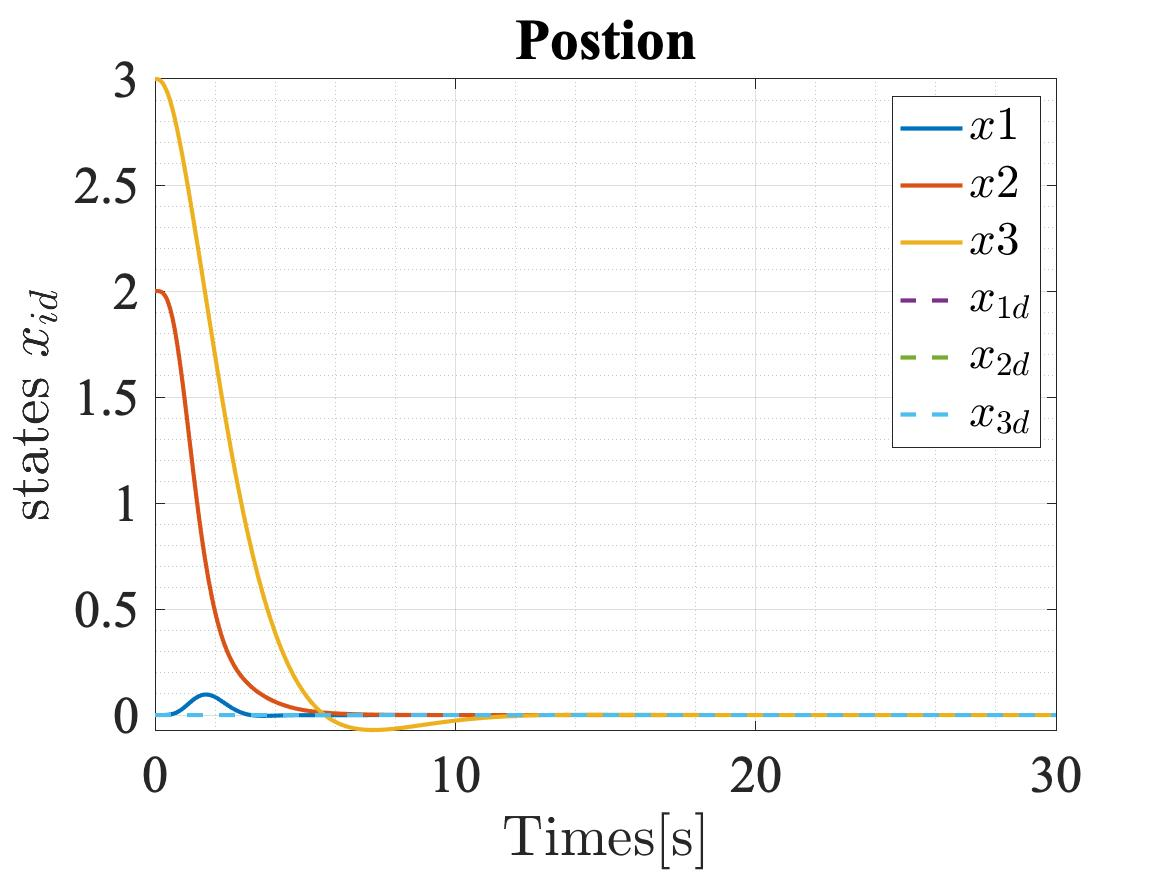
\includegraphics[width=1\textwidth]{Postion_T_LQR.jpg}
            \caption{Postion without disturbance}
        \end{figure}

        \column{0.5\textwidth}
        \begin{figure}[h]
            \centering
            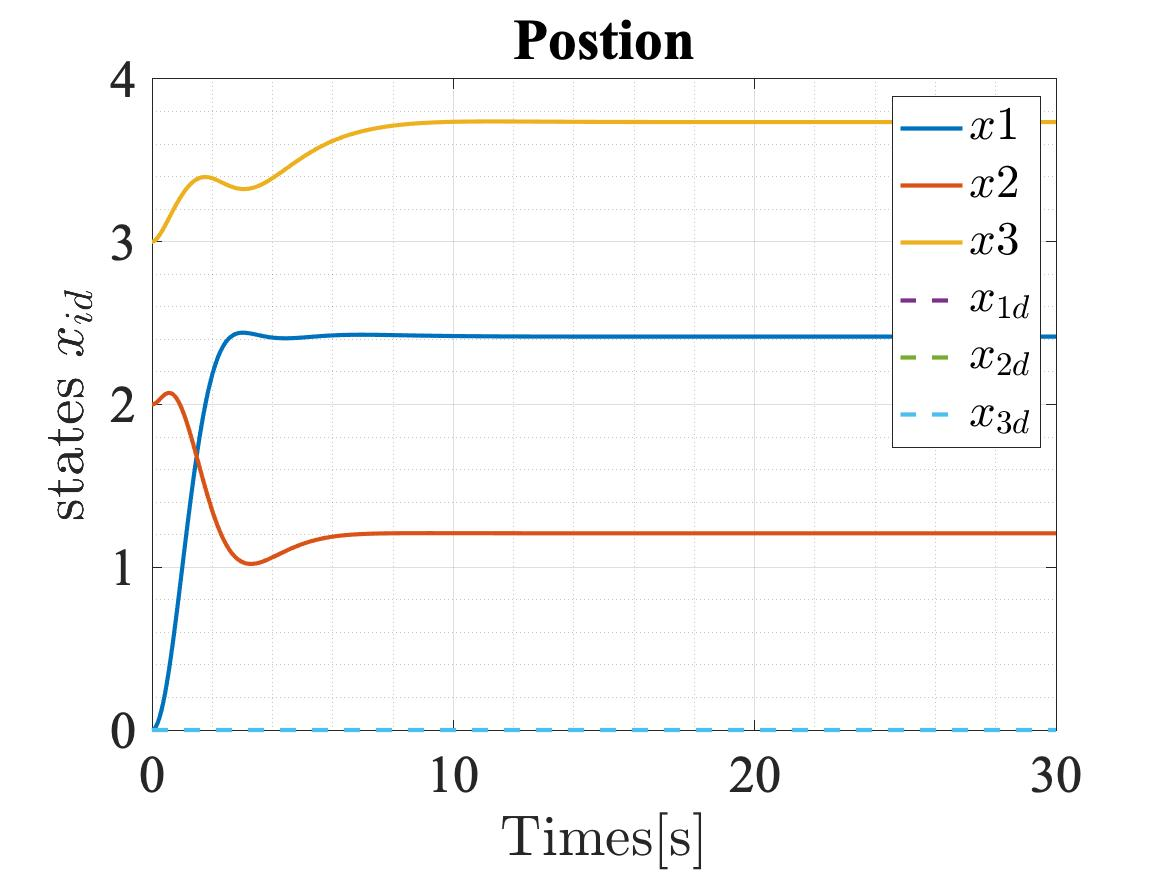
\includegraphics[width=1\textwidth]{Postion_T_LQR_Dist.jpg}
            \caption{Postion with disturbance}
        \end{figure}
    \end{columns}
\end{frame}
\begin{frame}
    \frametitle{Velocity}

    \begin{columns}

        \column{0.5\textwidth}
        \begin{figure}[h]
            \centering
            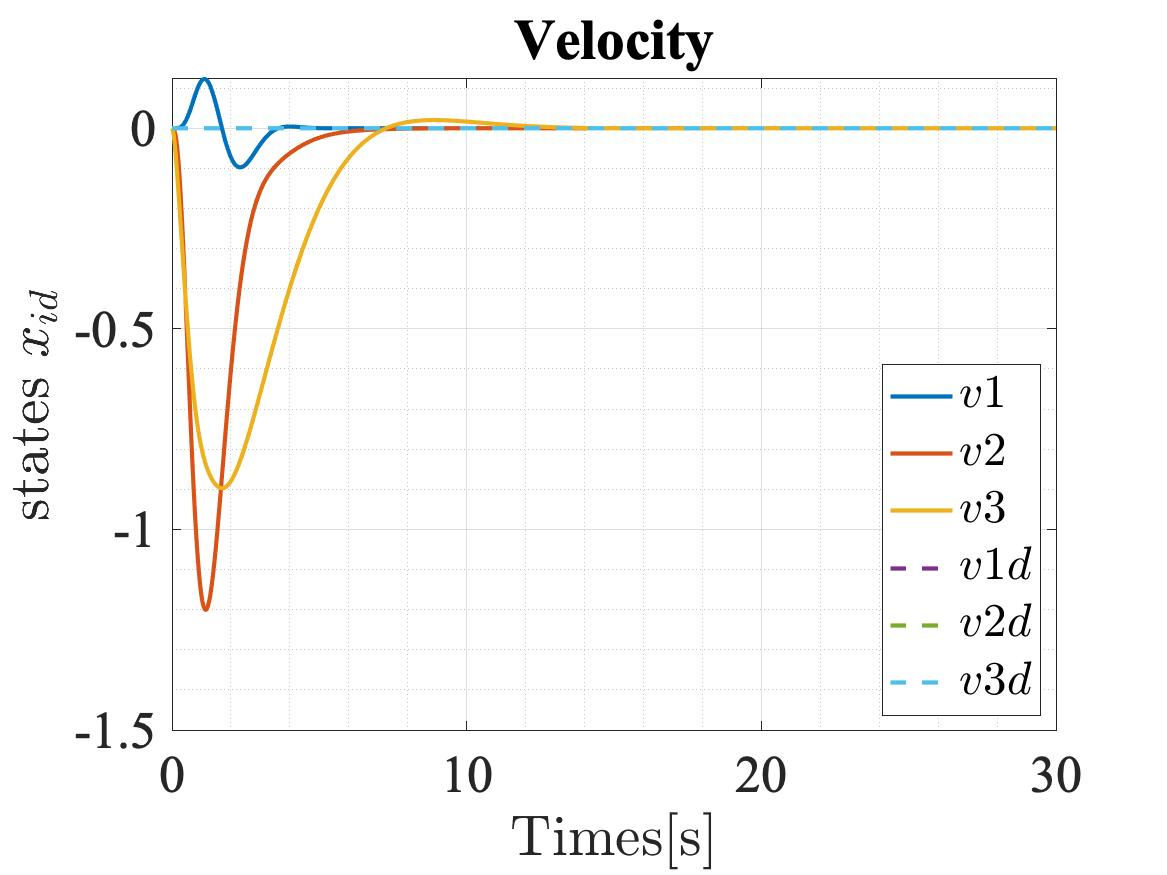
\includegraphics[width=1\textwidth]{Velocity_T_LQR.jpg}
            \caption{Velocity without disturbance}
        \end{figure}

        \column{0.5\textwidth}
        \begin{figure}[h]
            \centering
            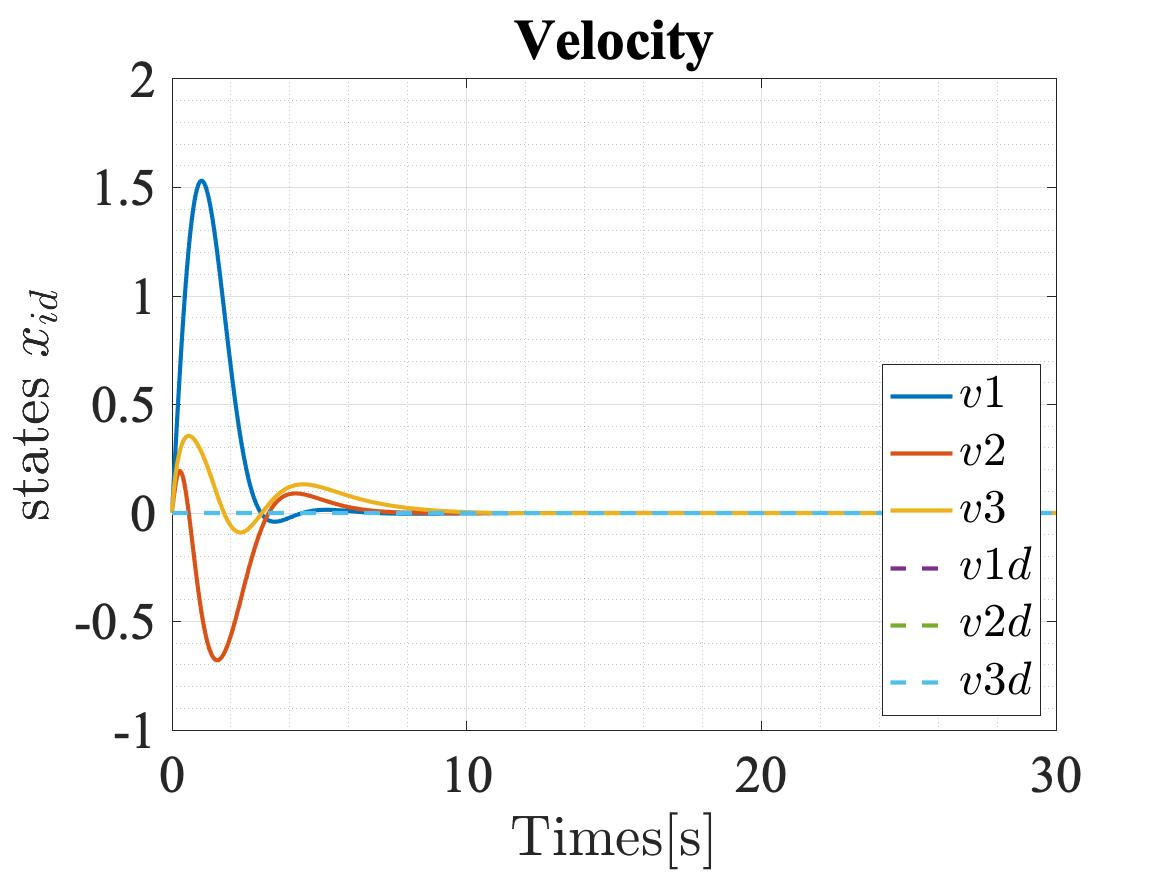
\includegraphics[width=1\textwidth]{Velocity_T_LQR_Dist.jpg}
            \caption{Velocity with disturbance}
        \end{figure}
    \end{columns}
\end{frame}
\begin{frame}
    \frametitle{Euler}

    \begin{columns}

        \column{0.5\textwidth}
        \begin{figure}[h]
            \centering
            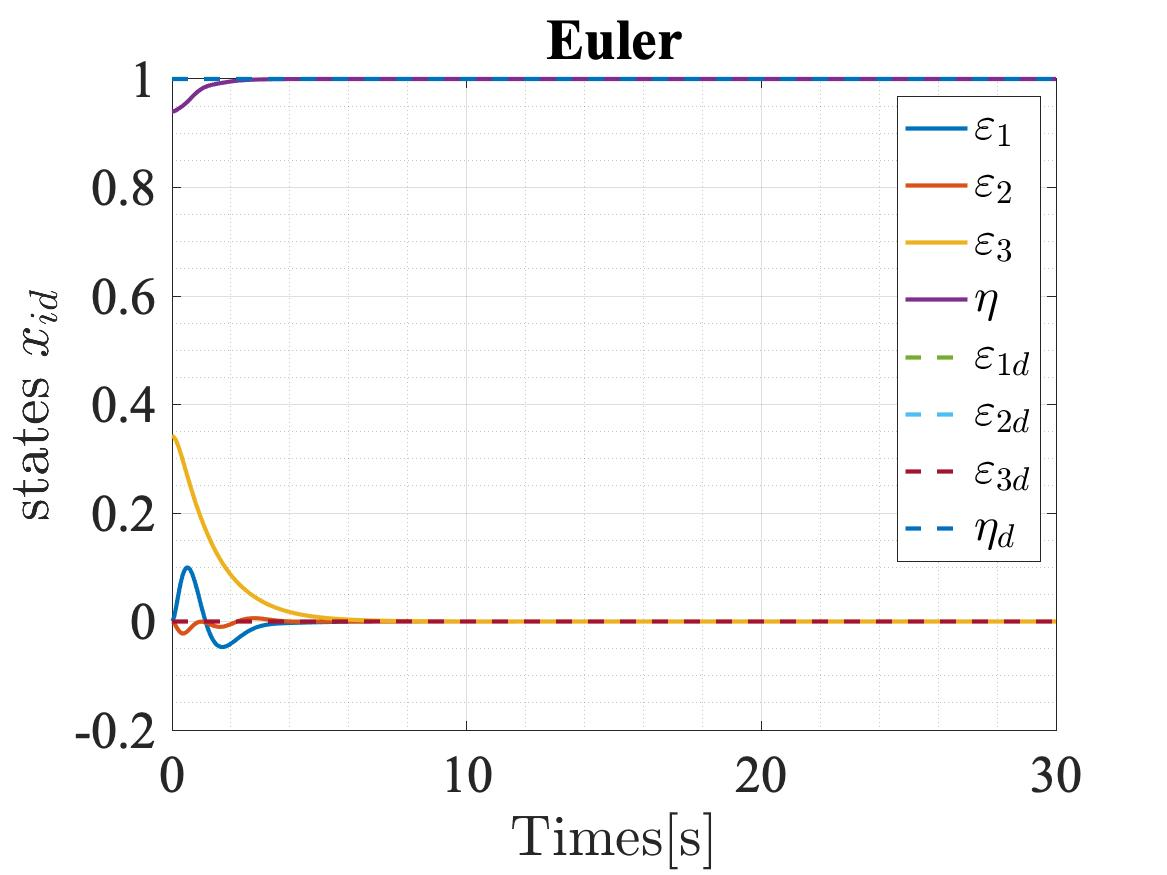
\includegraphics[width=1\textwidth]{Euler_T_LQR.jpg}
            \caption{Euler without disturbance}
        \end{figure}

        \column{0.5\textwidth}
        \begin{figure}[h]
            \centering
            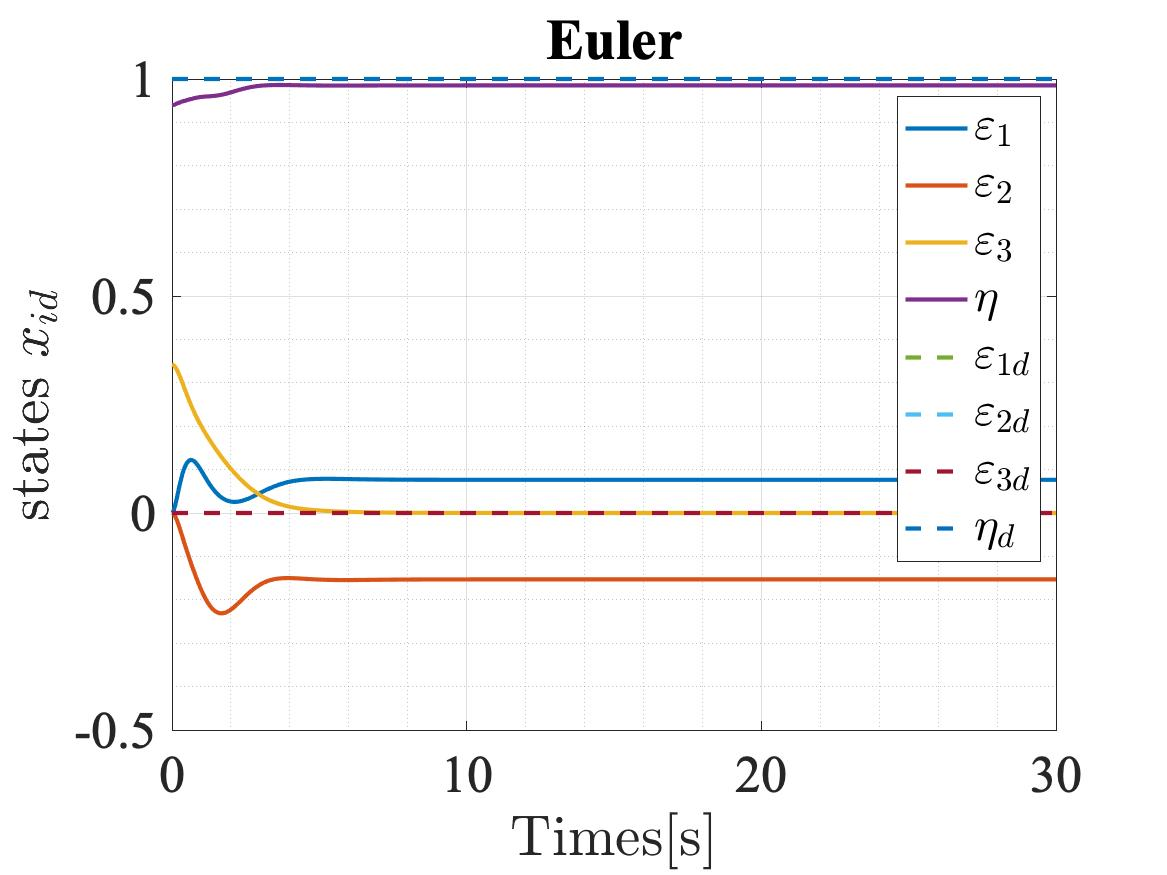
\includegraphics[width=1\textwidth]{Euler_T_LQR_Dist.jpg}
            \caption{Euler with disturbance}
        \end{figure}
    \end{columns}
\end{frame}
\begin{frame}
    \frametitle{Angular Velocity}


    \begin{columns}

        \column{0.5\textwidth}
        \begin{figure}[h]
            \centering
            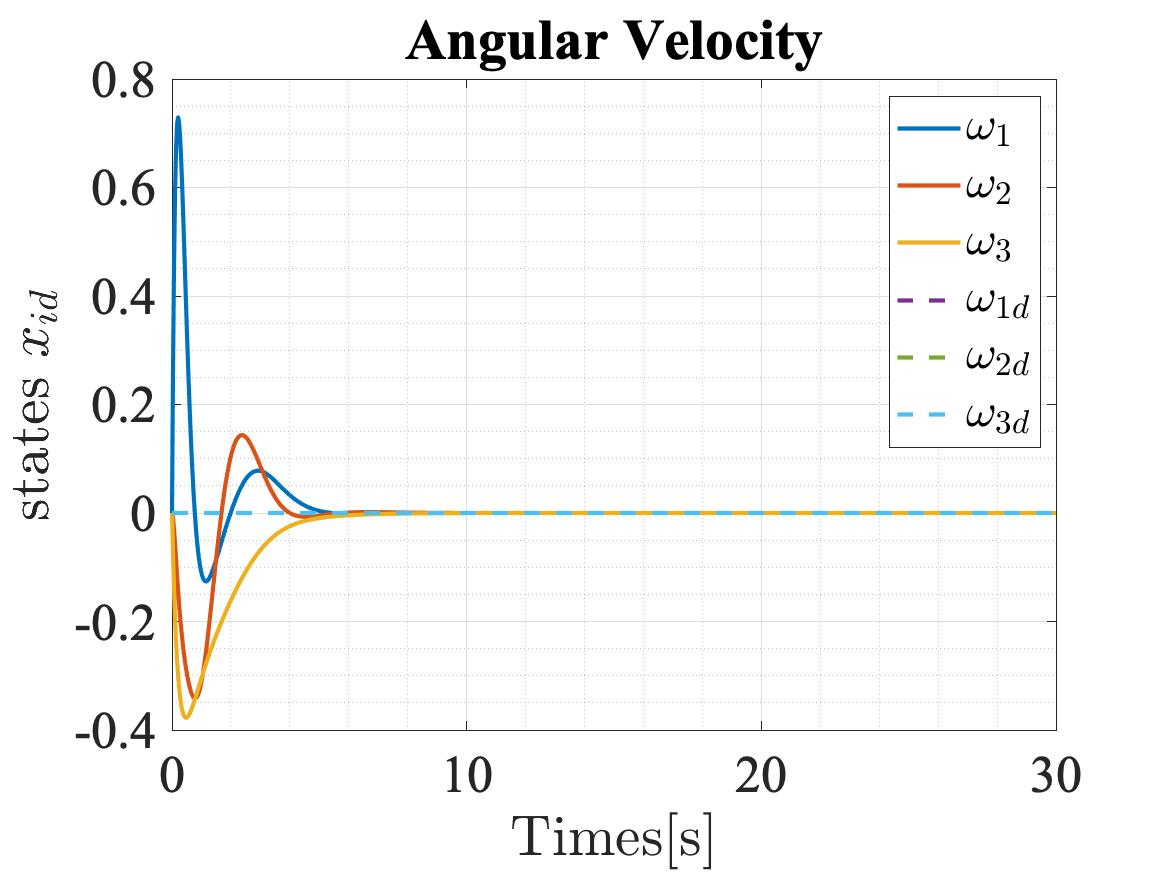
\includegraphics[width=1\textwidth]{Angular_Velociy_T_LQR_Dist.jpg}
            \caption{Angular Velocity without disturbance}
        \end{figure}

        \column{0.5\textwidth}
        \begin{figure}[h]
            \centering
            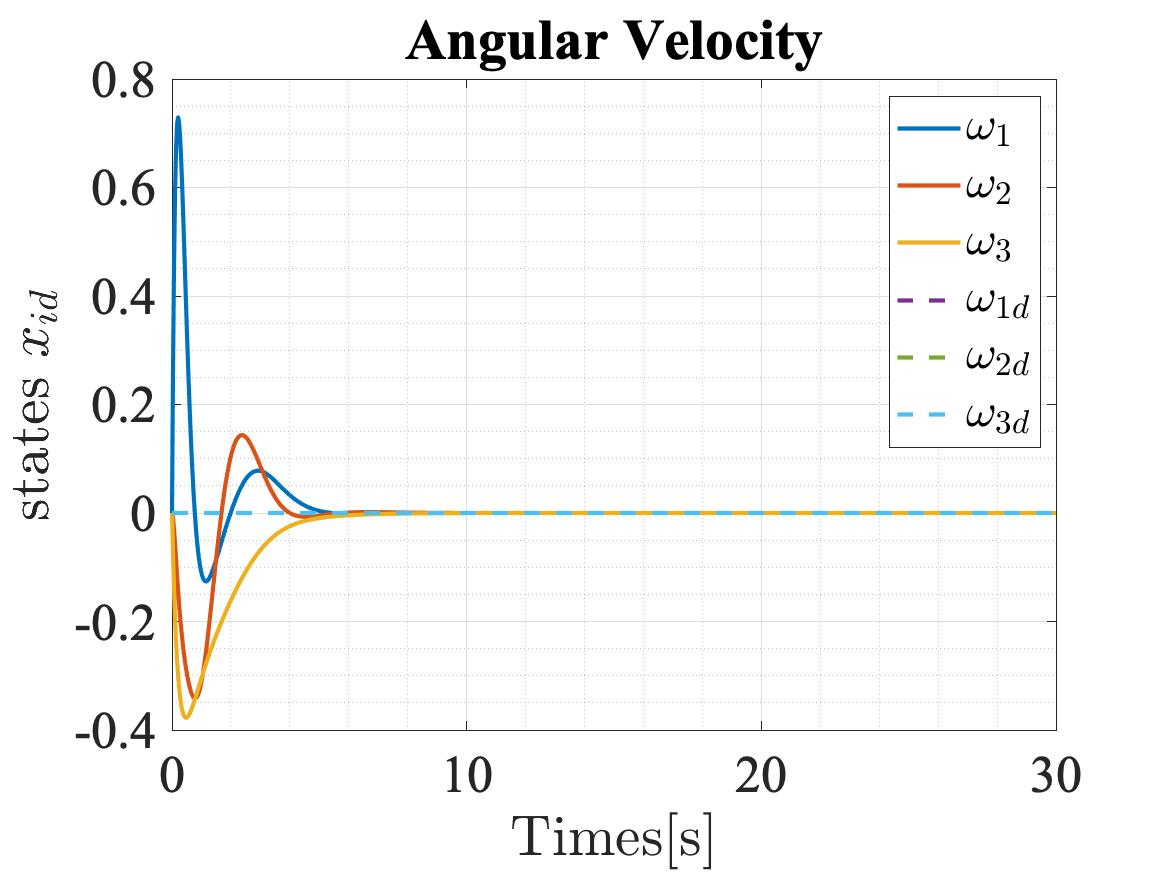
\includegraphics[width=1\textwidth]{Angular_Velociy_T_LQR_Dist.jpg}
            \caption{Angular Velocity with disturbance}
        \end{figure}
    \end{columns}

\end{frame}

\begin{frame}
    \frametitle{Thrust}

    \begin{columns}

        \column{0.5\textwidth}
        \begin{figure}[h]
            \centering
            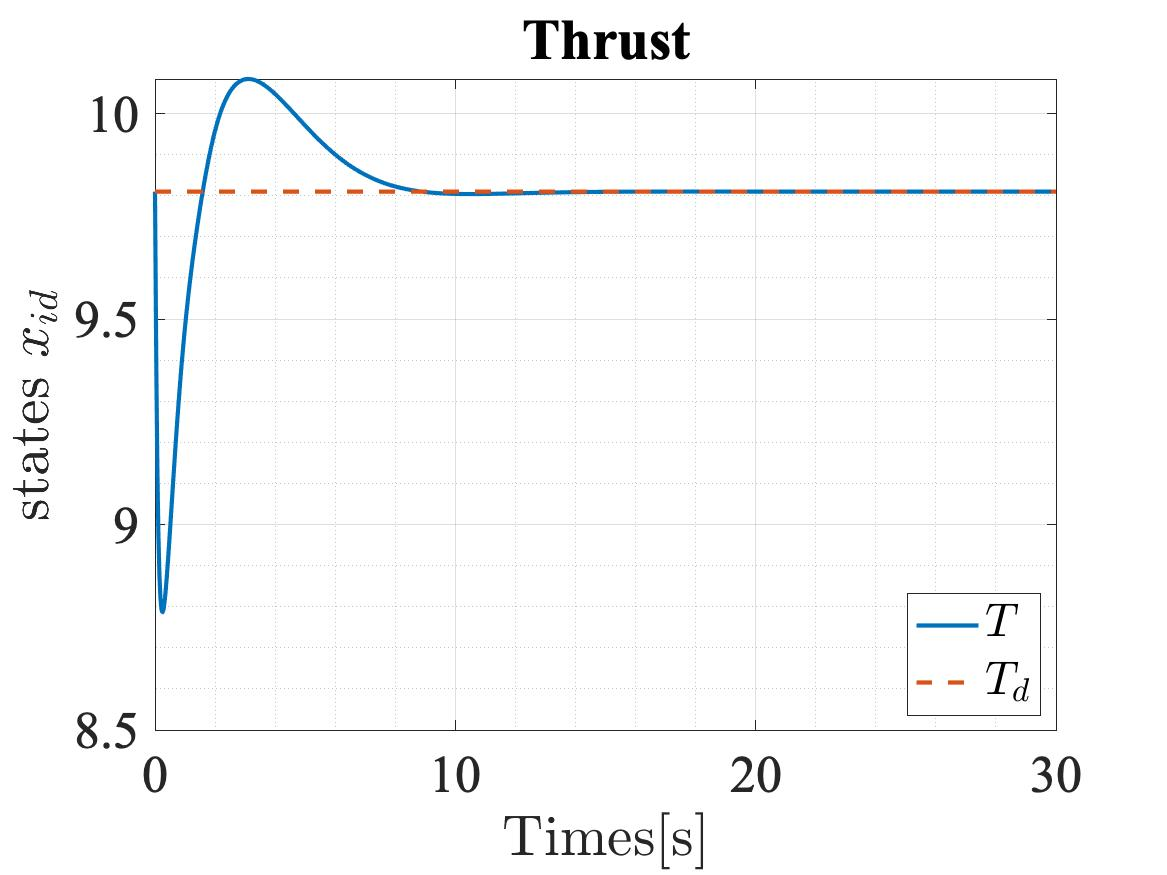
\includegraphics[width=1\textwidth]{Thrust_T_LQR.jpg}
            \caption{Thrust without disturbance}
        \end{figure}

        \column{0.5\textwidth}
        \begin{figure}[h]
            \centering
            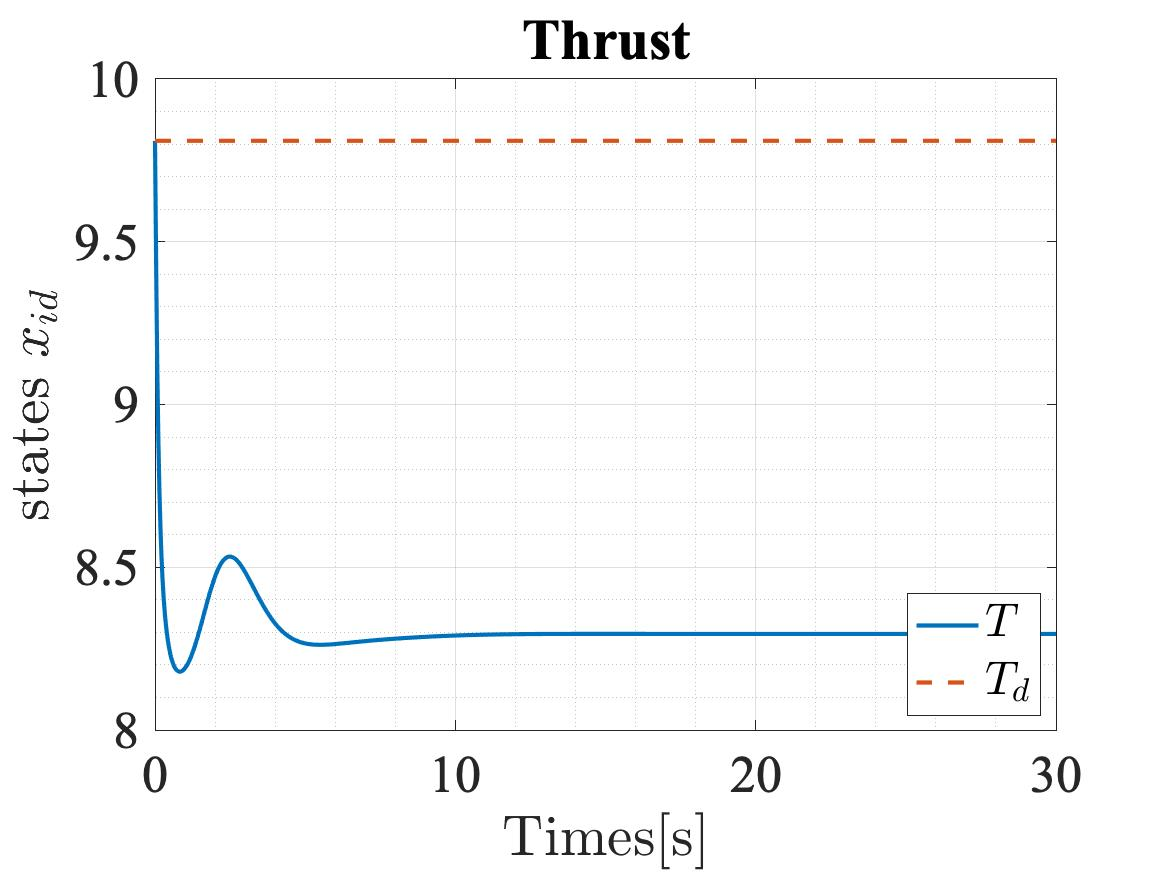
\includegraphics[width=1\textwidth]{Thrust_T_LQR_Dist.jpg}
            \caption{Thrust with disturbance}
        \end{figure}
    \end{columns}
\end{frame}
\begin{frame}
    \frametitle{Inputs}

    \begin{columns}

        \column{0.5\textwidth}
        \begin{figure}[h]
            \centering
            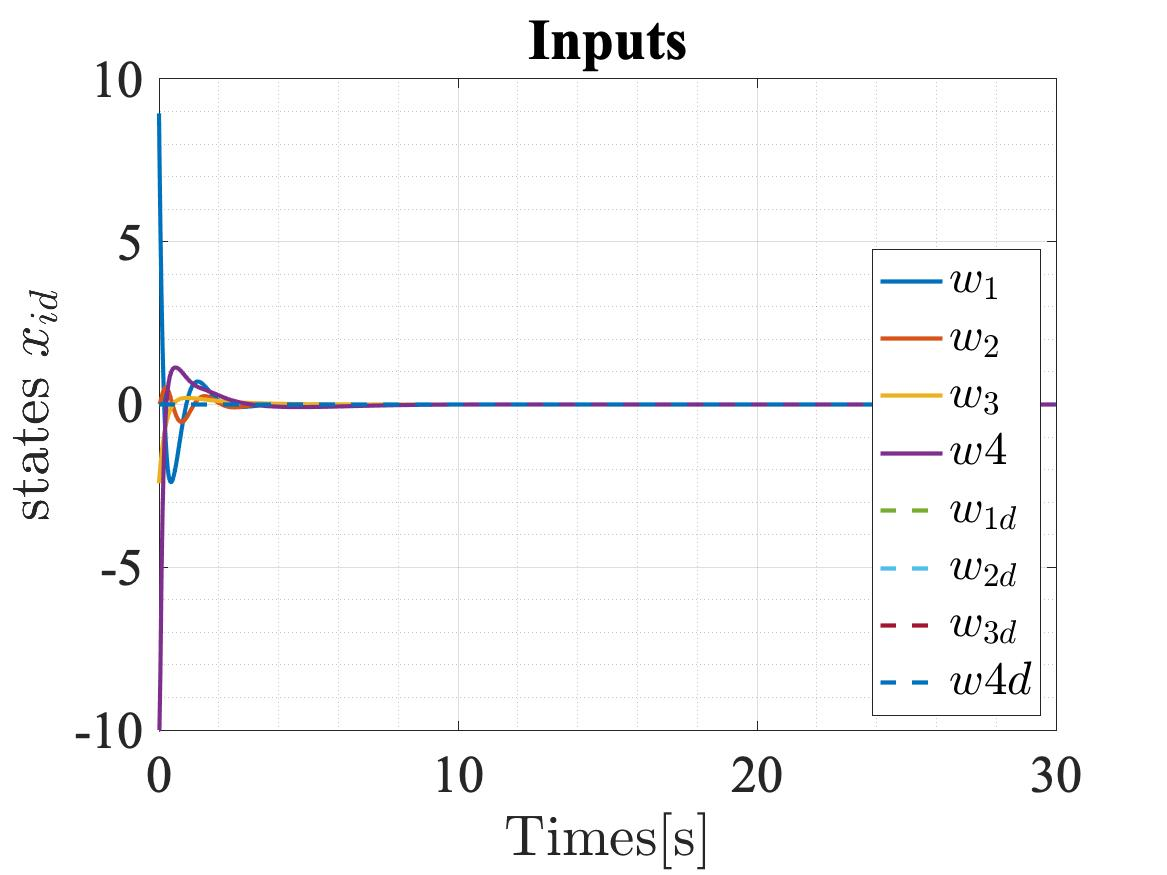
\includegraphics[width=1\textwidth]{Inputs_T_LQR.jpg}
            \caption{Inputs without disturbance}
        \end{figure}

        \column{0.5\textwidth}
        \begin{figure}[h]
            \centering
            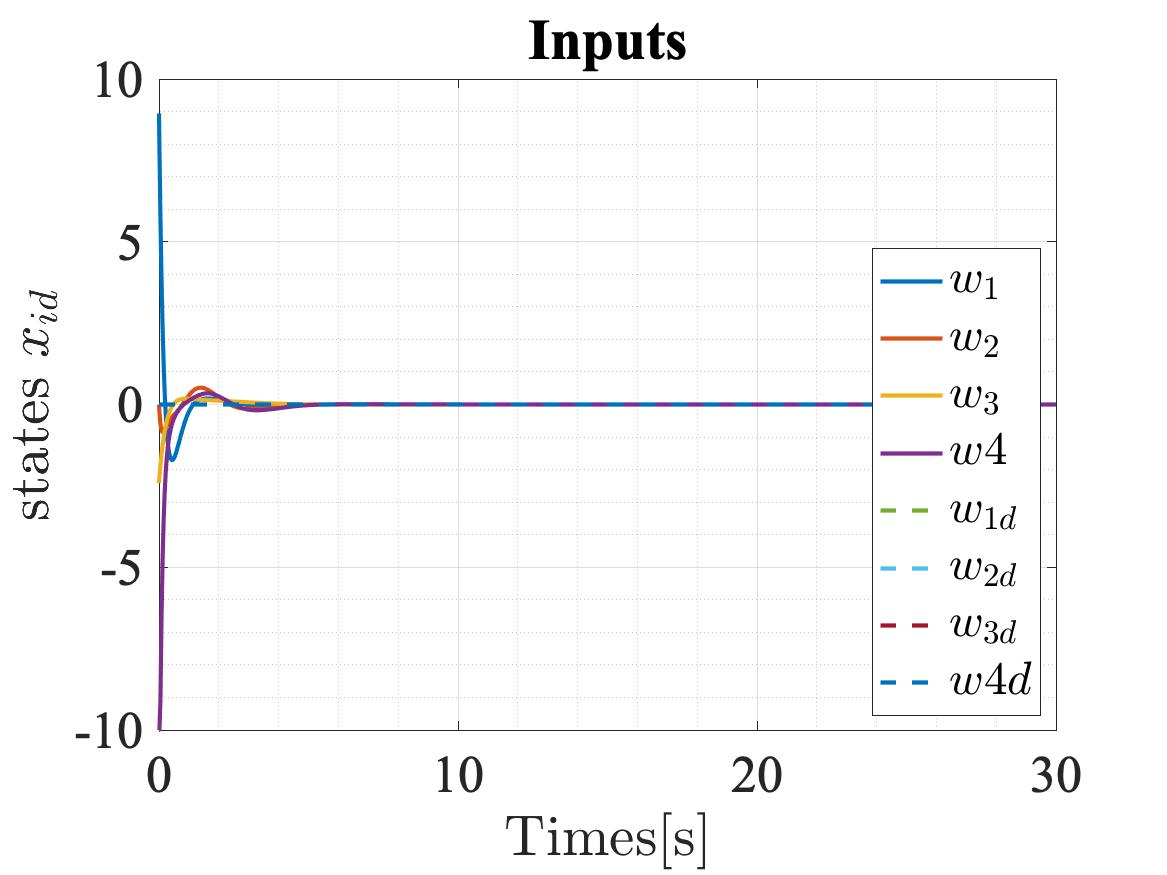
\includegraphics[width=1\textwidth]{Inputs_T_LQR_Dist.jpg}
            \caption{Inputs with disturbance}
        \end{figure}
    \end{columns}
\end{frame}

\subsection{Servo controller}
\begin{frame}

    Constant disturbance $\left(F_{d i s}=[2.50,1.25,2.00]^{T}\right)$ was added to the translational dynamics $(\dot{\boldsymbol{v}})$. The following figures show the outputs:
\end{frame}
\begin{frame}
    \frametitle{Postion}

    \begin{columns}

        \column{0.5\textwidth}
        \begin{figure}[h]
            \centering
            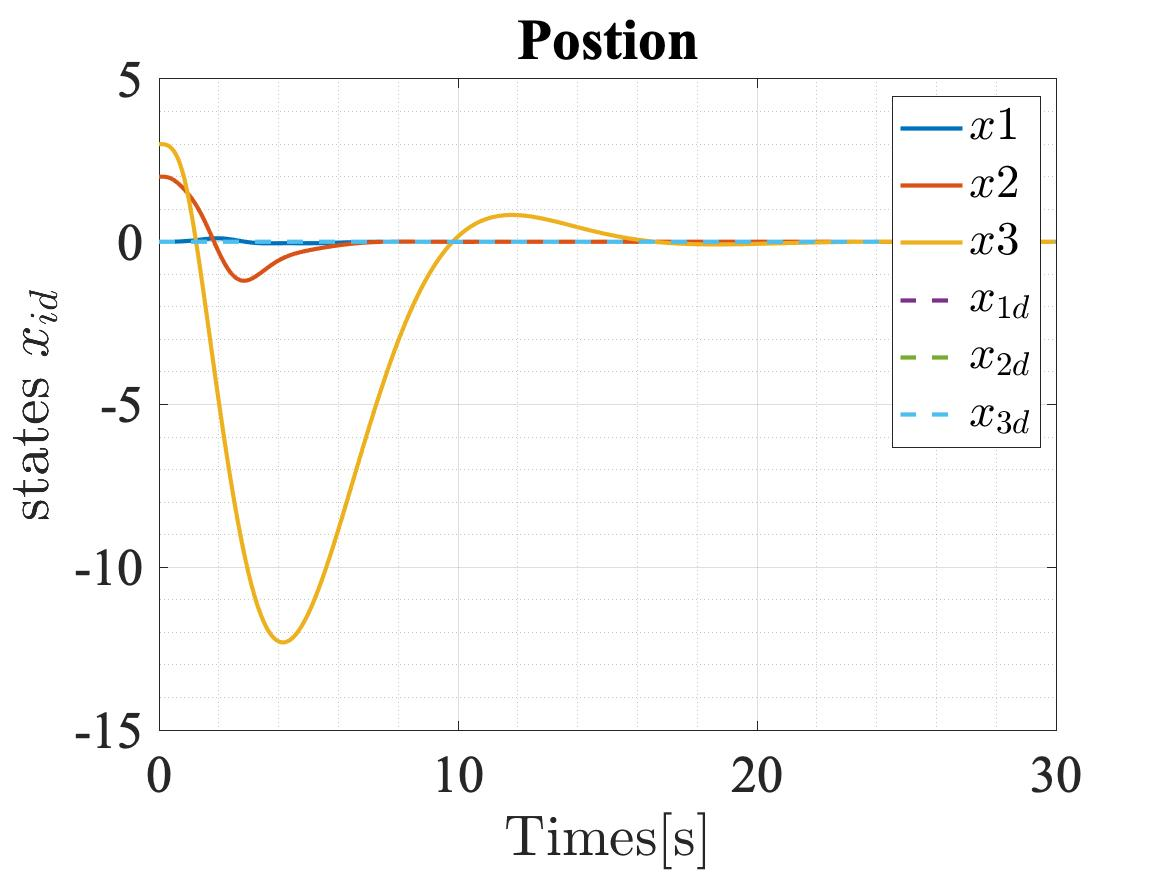
\includegraphics[width=1\textwidth]{Postion_T_Servo.jpg}
            \caption{Postion without disturbance}
        \end{figure}

        \column{0.5\textwidth}
        \begin{figure}[h]
            \centering
            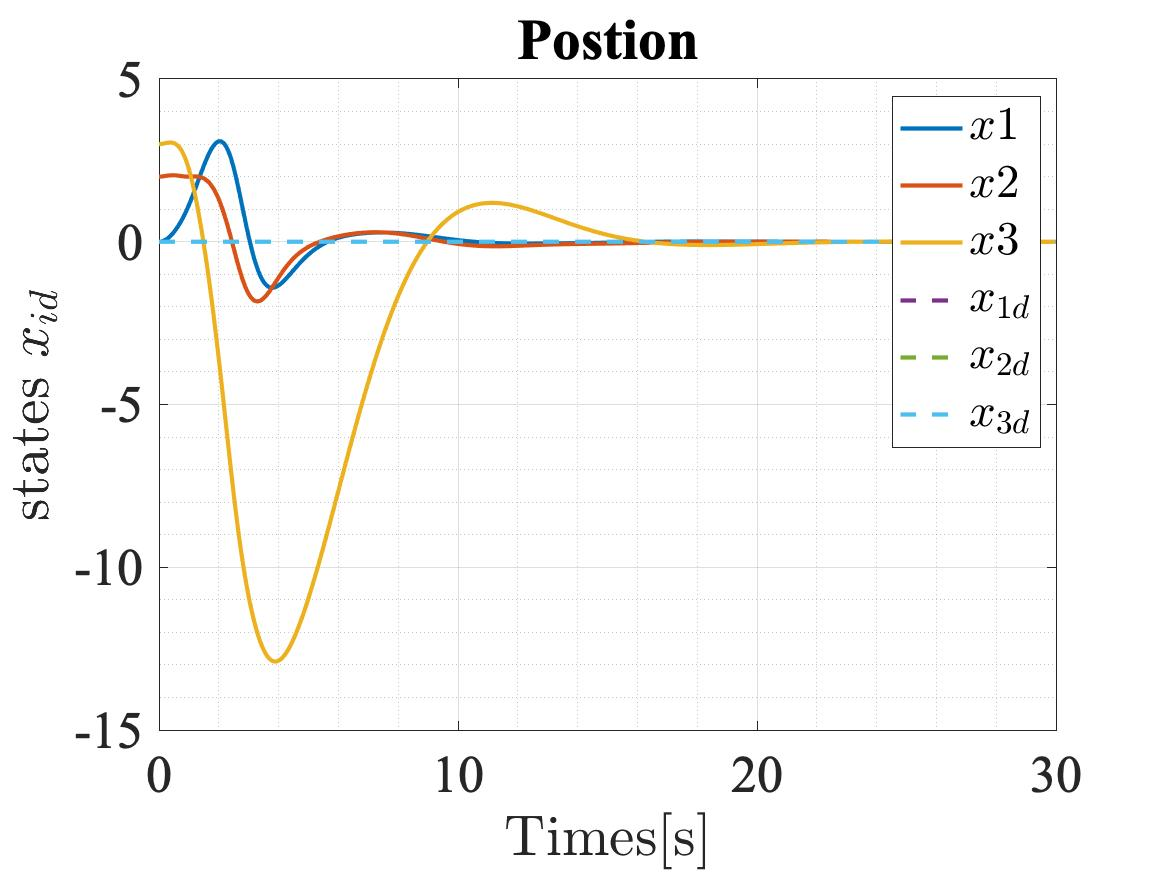
\includegraphics[width=1\textwidth]{Postion_T_Servo_Dist.jpg}
            \caption{Postion with disturbance}
        \end{figure}
    \end{columns}
\end{frame}
\begin{frame}
    \frametitle{Velocity}

    \begin{columns}

        \column{0.5\textwidth}
        \begin{figure}[h]
            \centering
            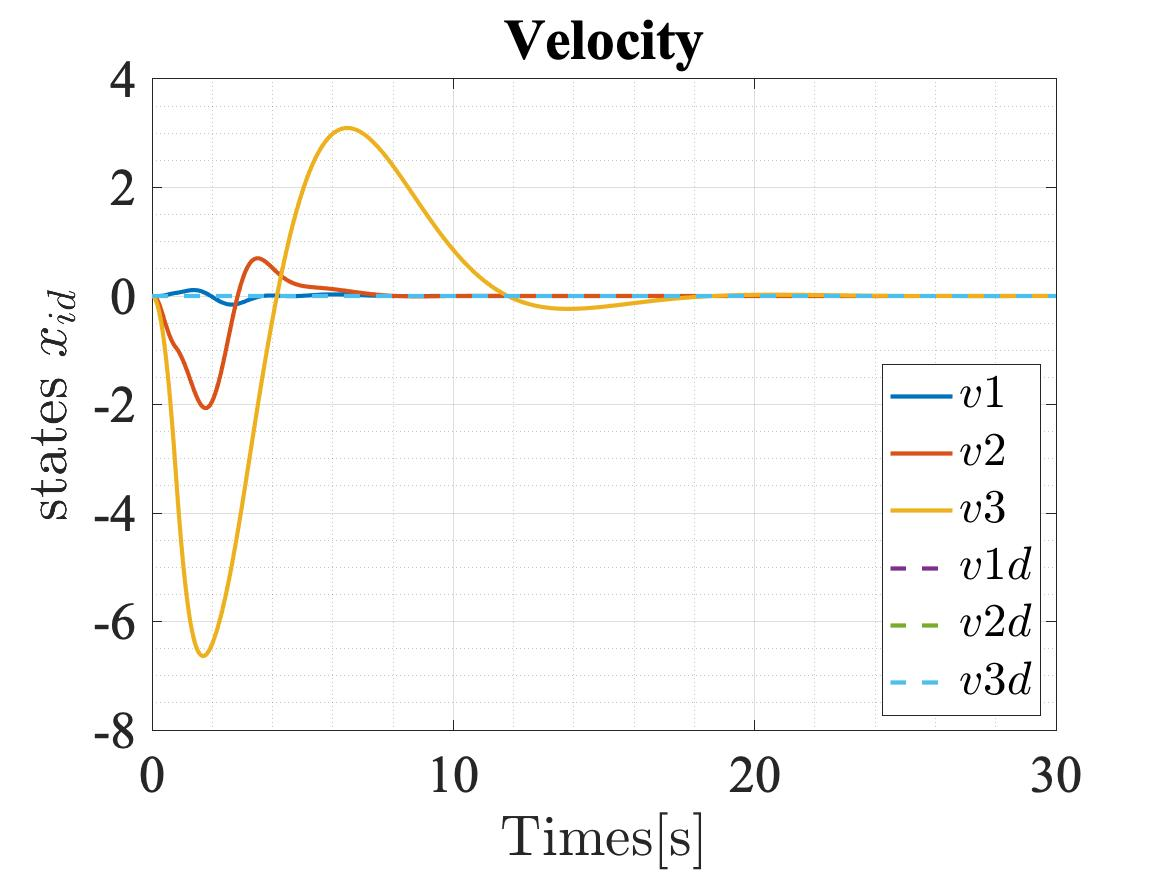
\includegraphics[width=1\textwidth]{Velocity_T_Servo.jpg}
            \caption{Velocity without disturbance}
        \end{figure}

        \column{0.5\textwidth}
        \begin{figure}[h]
            \centering
            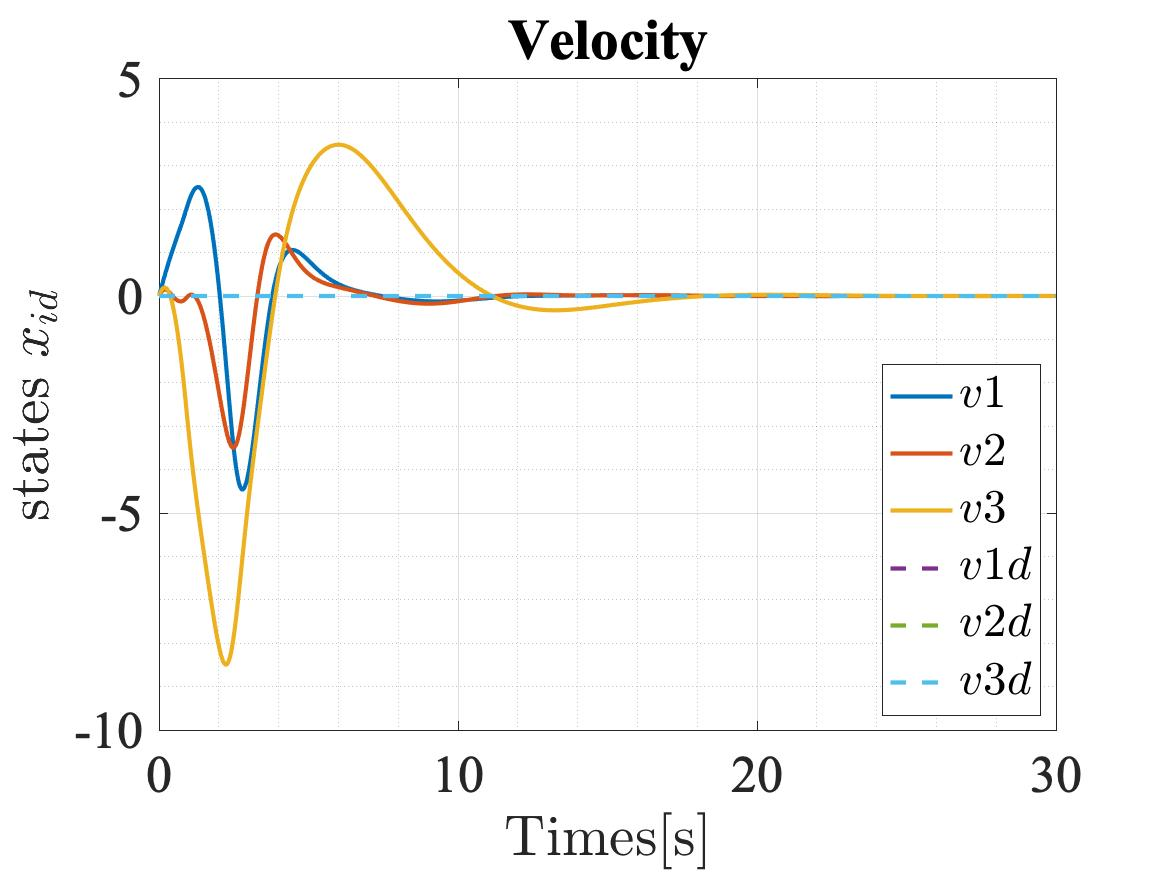
\includegraphics[width=1\textwidth]{Velocity_T_Servo_Dist.jpg}
            \caption{Velocity with disturbance}
        \end{figure}
    \end{columns}
\end{frame}
\begin{frame}
    \frametitle{Euler}

    \begin{columns}

        \column{0.5\textwidth}
        \begin{figure}[h]
            \centering
            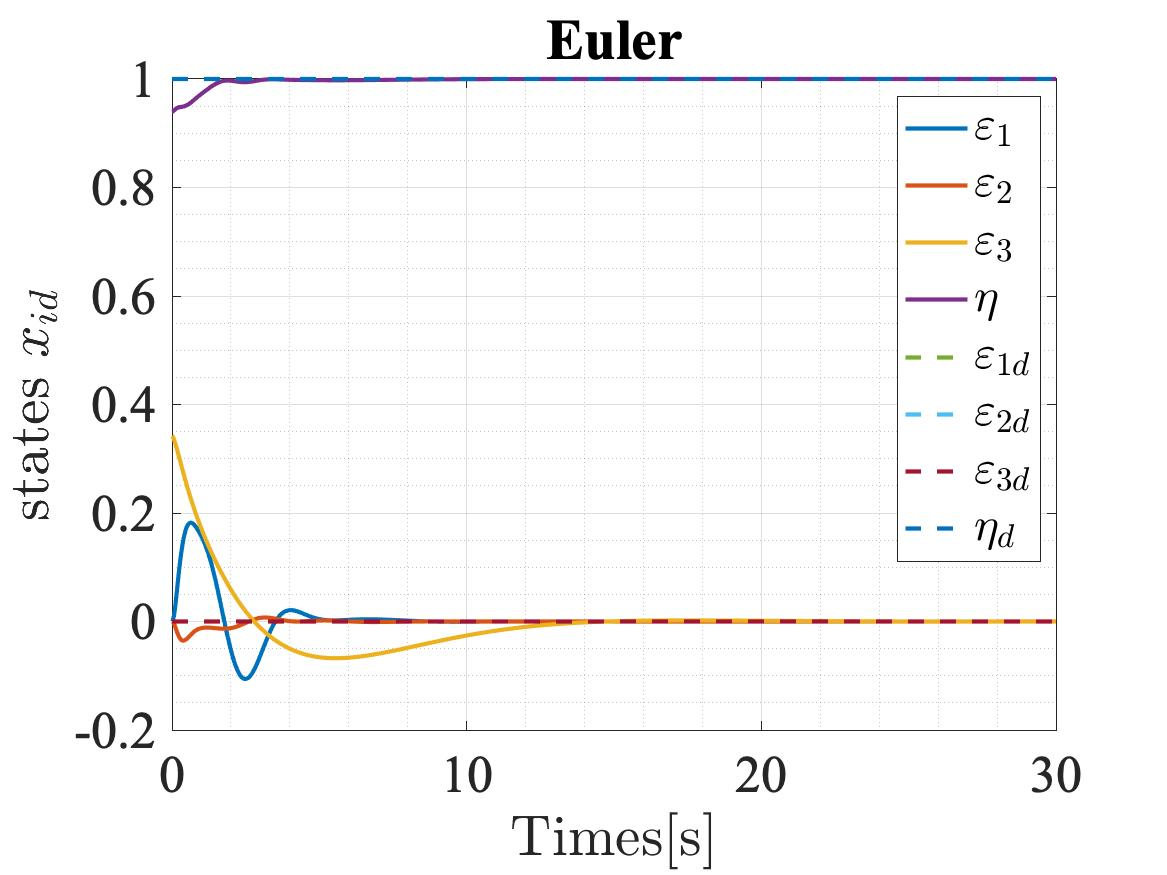
\includegraphics[width=1\textwidth]{Euler_T_Servo.jpg}
            \caption{Euler without disturbance}
        \end{figure}

        \column{0.5\textwidth}
        \begin{figure}[h]
            \centering
            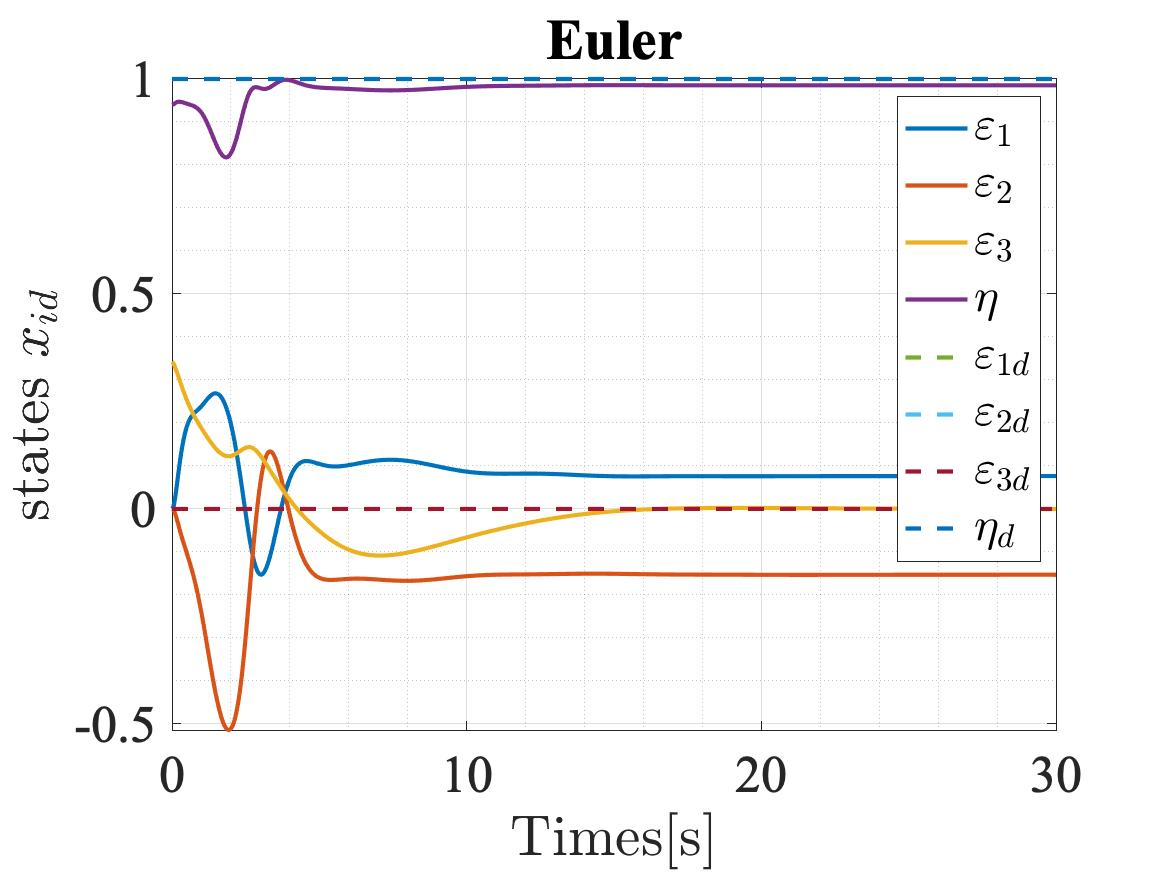
\includegraphics[width=1\textwidth]{Euler_T_Servo_Dist.jpg}
            \caption{Euler with disturbance}
        \end{figure}
    \end{columns}
\end{frame}
\begin{frame}
    \frametitle{Angular Velocity}


    \begin{columns}

        \column{0.5\textwidth}
        \begin{figure}[h]
            \centering
            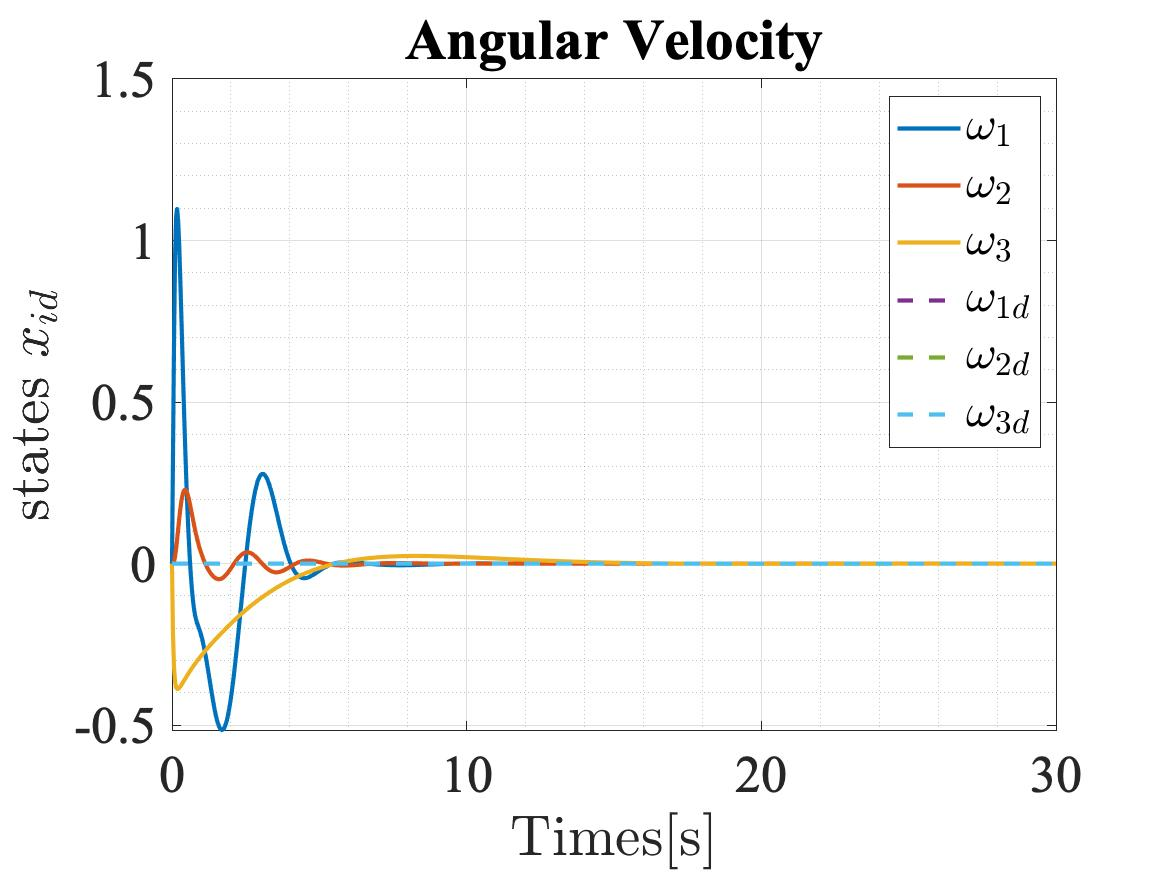
\includegraphics[width=1\textwidth]{Angular_Velociy_T_Servo.jpg}
            \caption{Angular Velocity without disturbance}
        \end{figure}

        \column{0.5\textwidth}
        \begin{figure}[h]
            \centering
            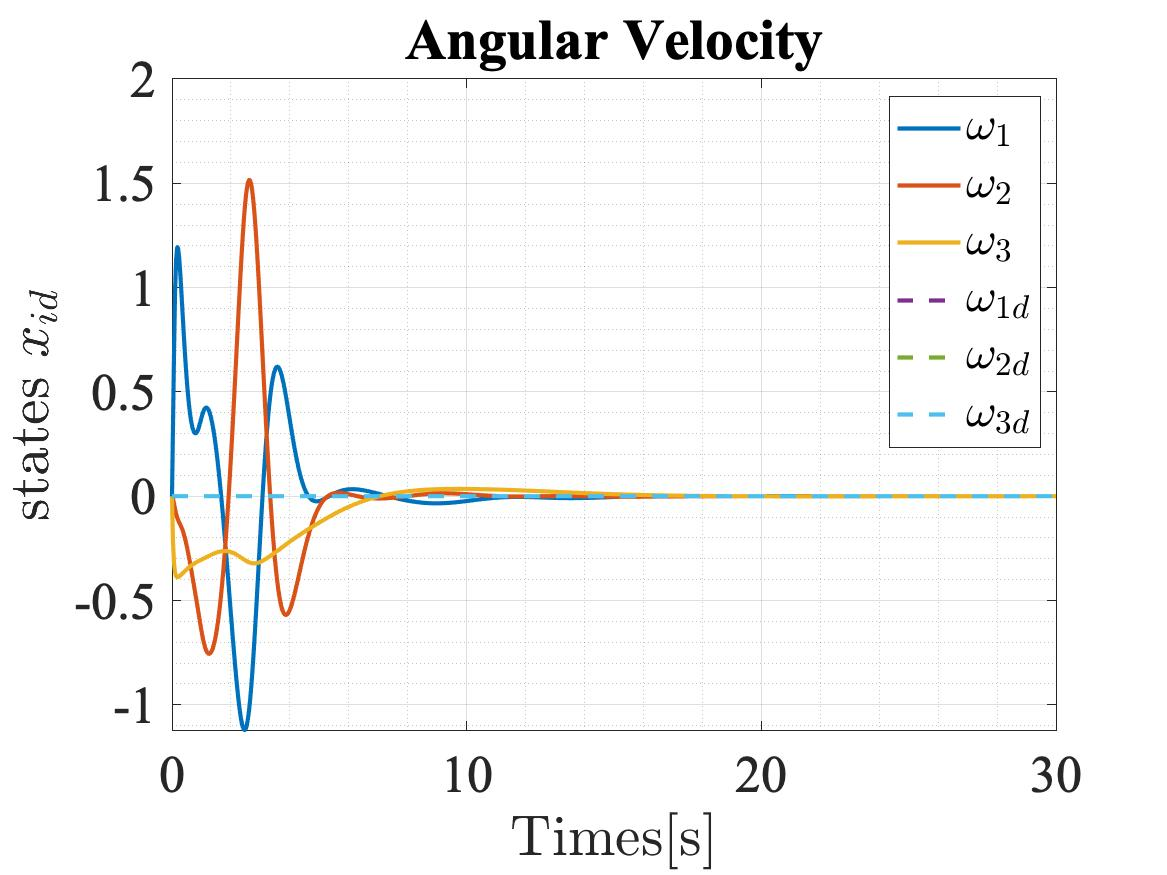
\includegraphics[width=1\textwidth]{Angular_Velociy_T_Servo_Dist.jpg}
            \caption{Angular Velocity with disturbance}
        \end{figure}
    \end{columns}

\end{frame}
\begin{frame}
    \frametitle{Thrust}

    \begin{columns}

        \column{0.5\textwidth}
        \begin{figure}[h]
            \centering
            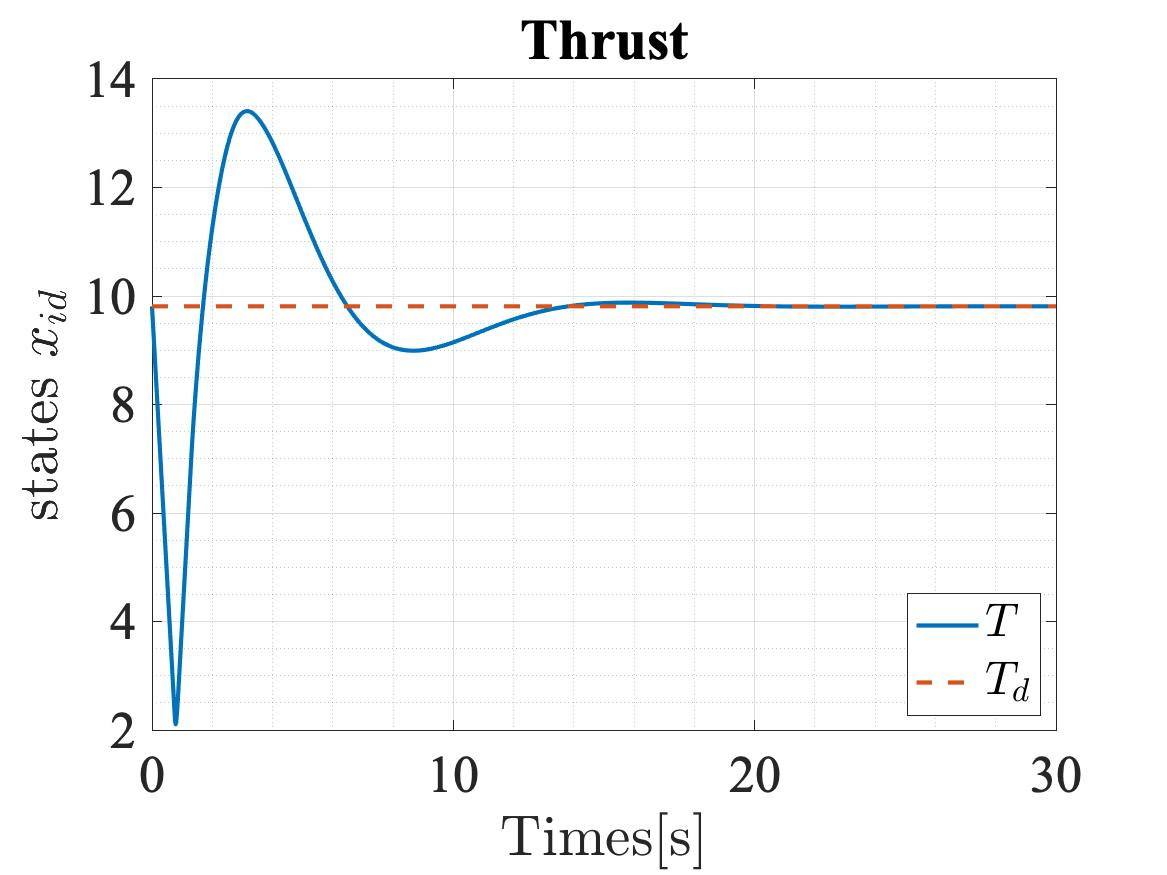
\includegraphics[width=1\textwidth]{Thrust_T_Servo.jpg}
            \caption{Thrust without disturbance}
        \end{figure}

        \column{0.5\textwidth}
        \begin{figure}[h]
            \centering
            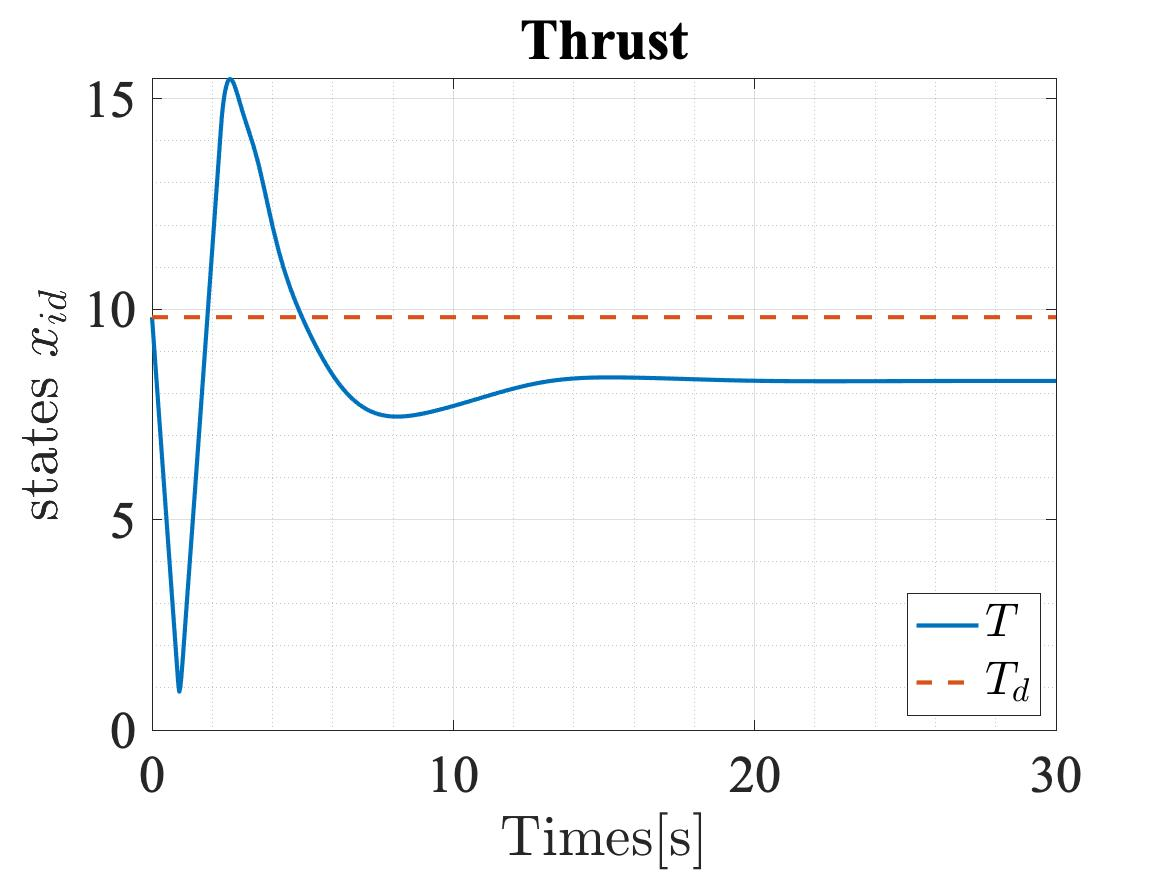
\includegraphics[width=1\textwidth]{Thrust_T_Servo_Dist.jpg}
            \caption{Thrust with disturbance}
        \end{figure}
    \end{columns}
\end{frame}

\begin{frame}
    \frametitle{Inputs}

    \begin{columns}

        \column{0.5\textwidth}
        \begin{figure}[h]
            \centering
            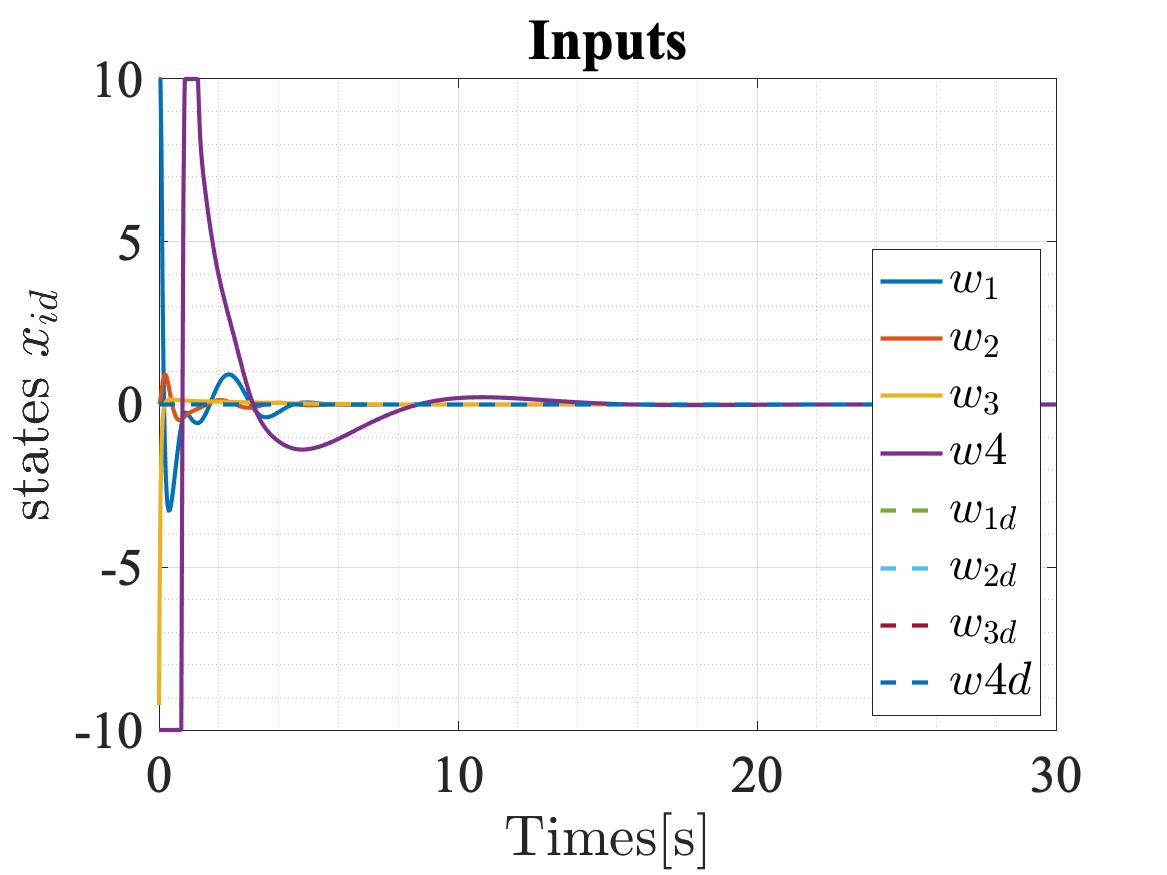
\includegraphics[width=1\textwidth]{Inputs_T_Servo.jpg}
            \caption{Inputs without disturbance}
        \end{figure}

        \column{0.5\textwidth}
        \begin{figure}[h]
            \centering
            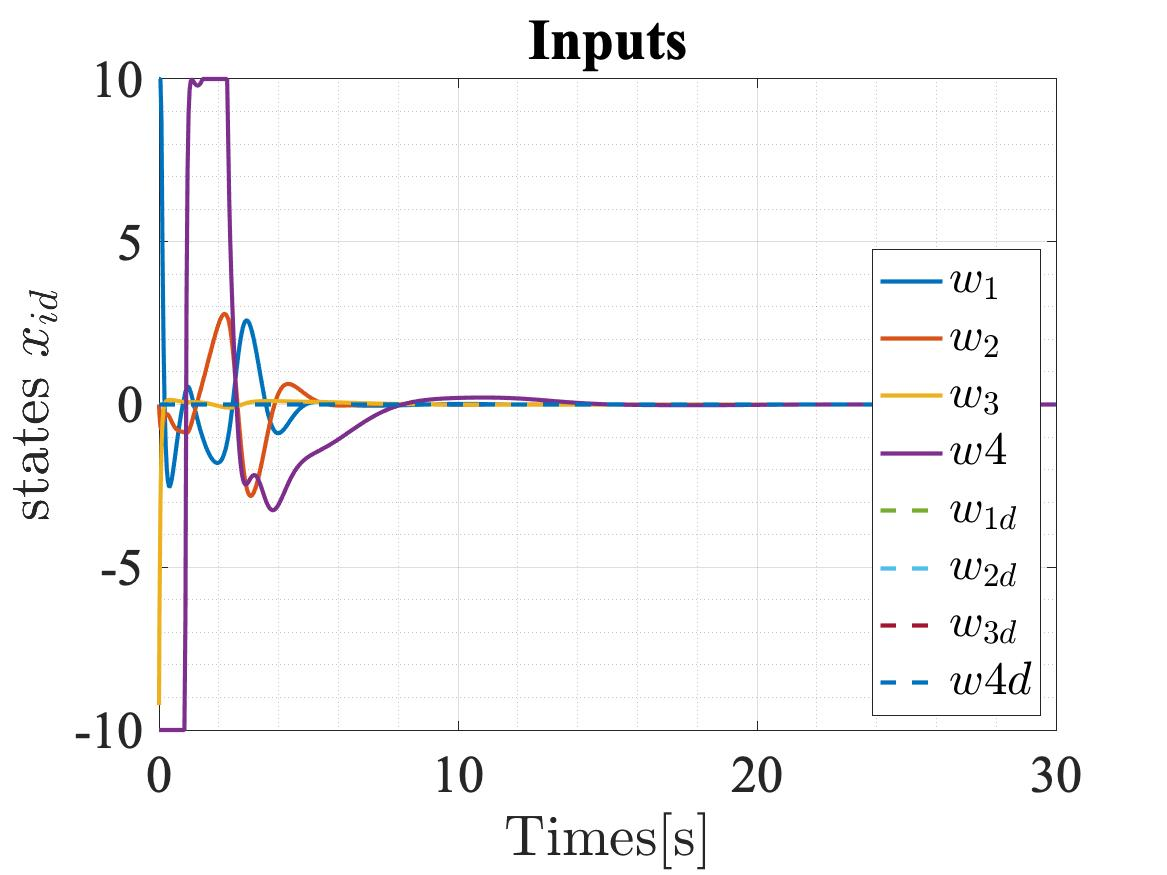
\includegraphics[width=1\textwidth]{Inputs_T_Servo_Dist.jpg}
            \caption{Inputs with disturbance}
        \end{figure}
    \end{columns}
\end{frame}


\end{document}